\chapter{\textsc{Système d'horloges}}

Comme tout système numérique, le microcontrôleur et ses périphériques ont besoin d'une horloge. Ce signal contrôle toutes les bascules composant les différentes machines séquentielles qui composent le système numérique. La structure détaillée de ce type de circuit séquentiel est étudiée au cours "Systèmes Logiques".

Le signal d'horloge est toujours généré par un oscillateur, dont les performances définissent les qualités:
\begin{itemize}[label=\textbullet,font=\small]
\item fréquence;
\item précision;
\item stabilité.
\end{itemize}

\section{Oscillateurs}
On distingue 4 types d'oscillateur. Ceux-ci se différencient par le mécanisme donnant naissance à l'oscillation et par les composants externes mis en oeuvre:
\begin{itemize}[label=\textbullet,font=\small]
\item oscillateurs RC (consulter le cours de "Electronique Analogique");
\item oscillateurs à résonateur céramique ou à quartz;
\item circuits oscillateurs spécifiques, éventuellement calibrés en usine et à compensation des effets de température;
\item circuits calés sur des signaux externes tels que GPS, dont la précision est obtenue par des horloges atomiques.
\end{itemize}

Dans les microcontrôleurs, on rencontre les deux premiers types.
Très souvent, un multiplicateur de fréquence permet de générer une horloge à plus haute fréquence que ce que les oscillateurs produisent.

\subsection{Oscillateurs RC}
L'oscillateur RC le plus simple est probablement celui illustré à la figure \ref{fig:Osc_RC_1}. Il est basé sur un inverseur logique à hystérèse ou \textit{Trigger de Schmitt}, une résistance et une capacité.

\begin{figure}[htb]
  \centering
  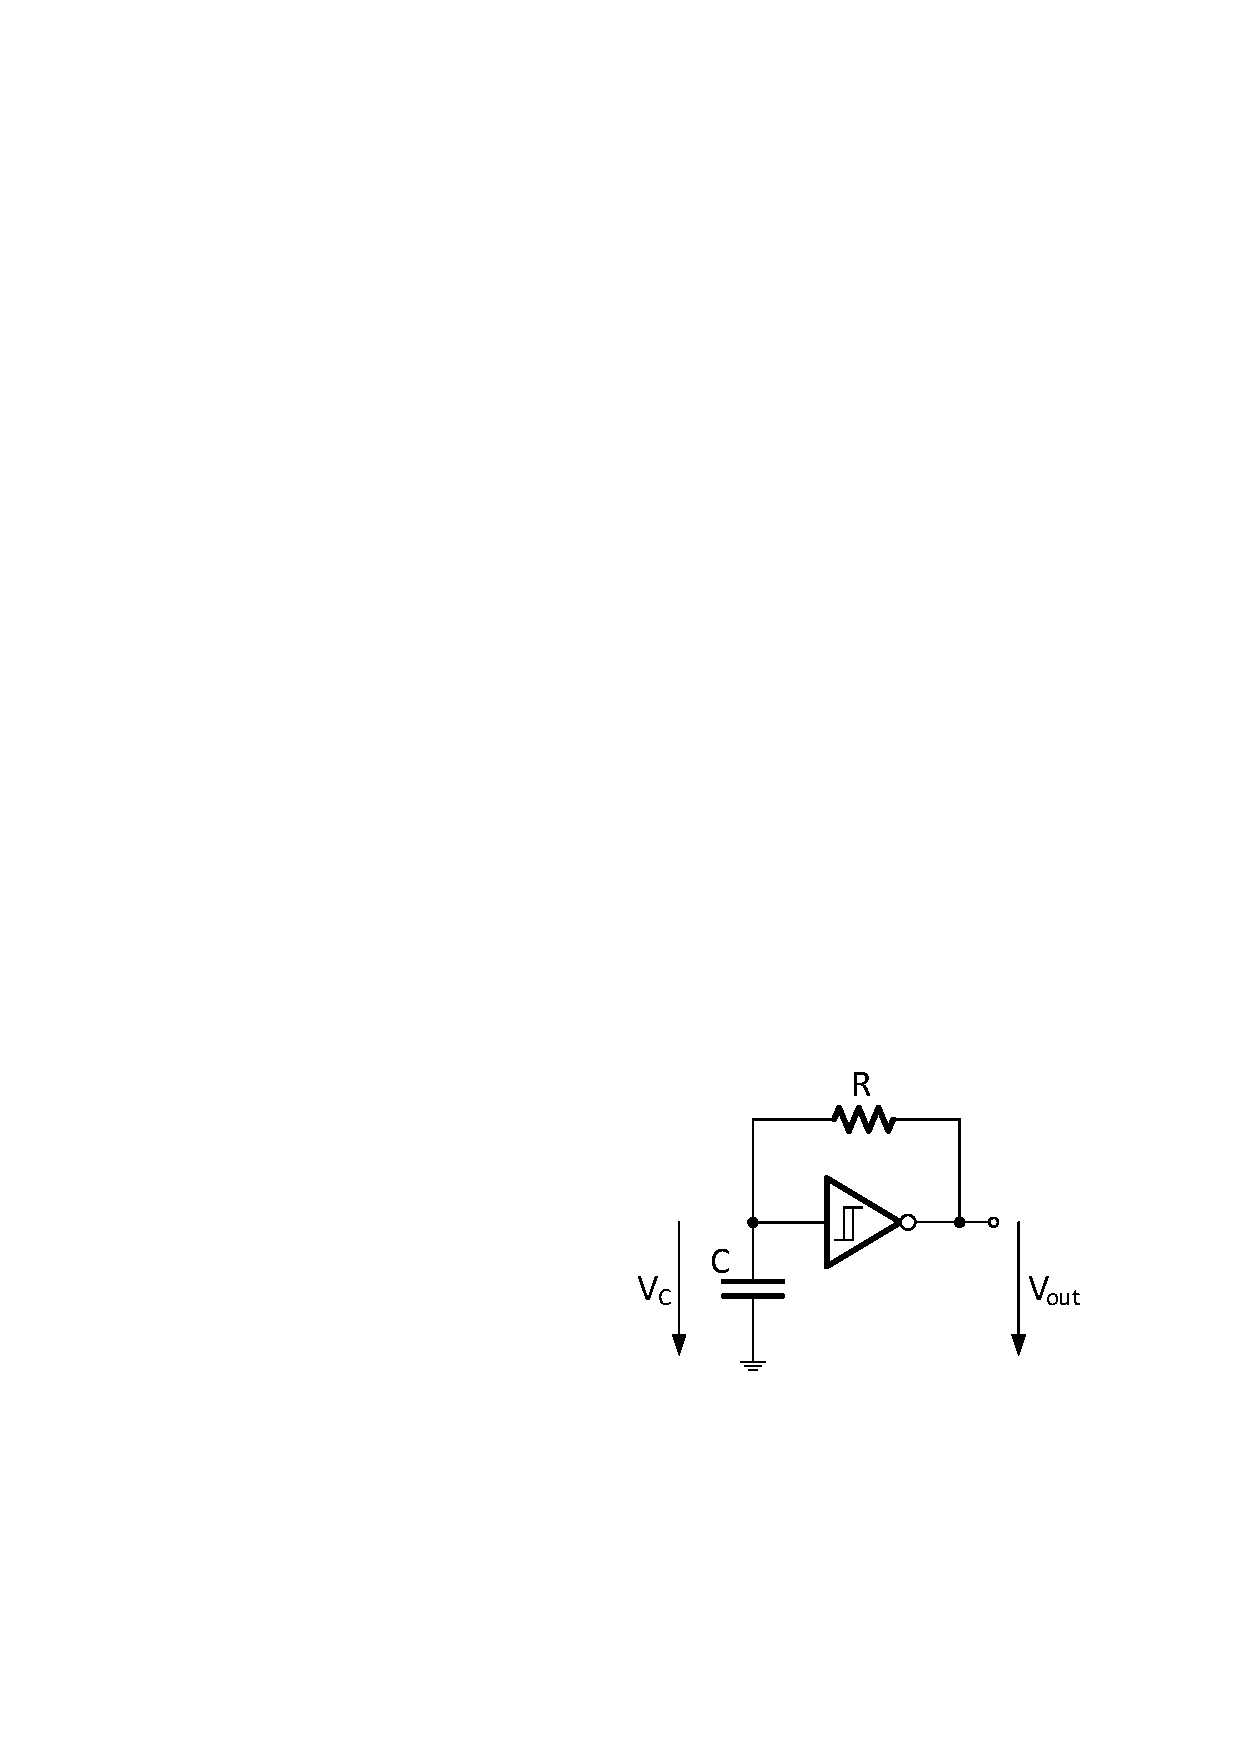
\includegraphics [angle=0, width=8cm]{./Figures/Chap6_Horloges/Osc_RC_1.pdf}
  \rule{35em}{0.5pt}
  \caption{Oscillateur RC à Trigger de Schmitt}
  \label{fig:Osc_RC_1}
\end{figure}

La figure \ref{fig:Osc_RC_2} illustre les signaux à l'entrée et à la sortie de l'inverseur à hystérèse.

\begin{figure}[htb]
  \centering
  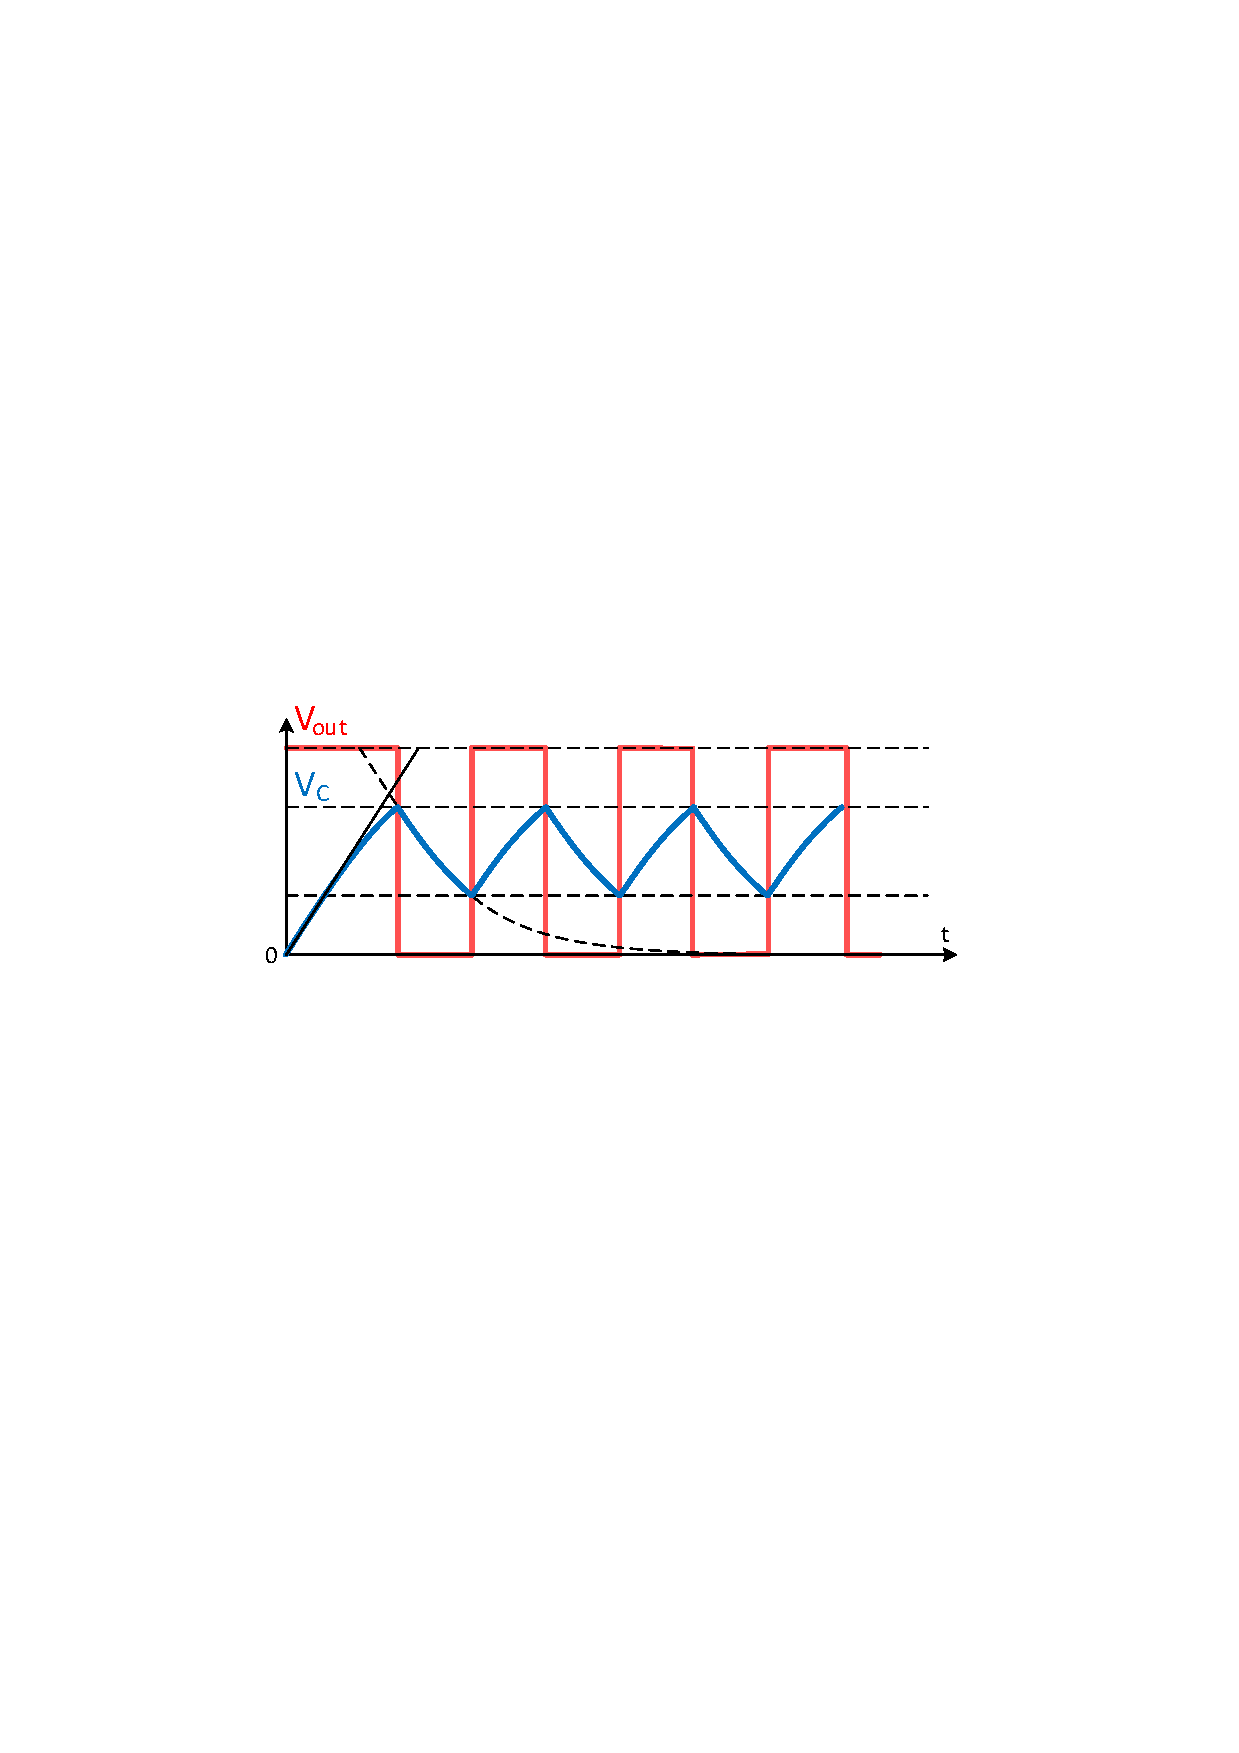
\includegraphics [angle=0, width=14cm]{./Figures/Chap6_Horloges/Osc_RC_2.pdf}
  \rule{35em}{0.5pt}
  \caption{Signal de l'oscillateur RC}
  \label{fig:Osc_RC_2}
\end{figure}

Du fait de la faible précision de la valeur des composants, tant la résistance, la capacité que les seuils d'hystérèse, la fréquence de l'oscillation est peu précise et peu stable en température. De plus, elle dépend de la tension d'alimentation. Par contre, tous les composants peuvent être intégrés. C'est pourquoi on rencontre ce type d'oscillateur dans la plupart des microcontrôleurs modernes, pour toutes les applications qui ne nécessitent pas une fréquence précise.

\subsection{Oscillateurs à quartz}
Si la fréquence doit être précise, l'oscillateur à quartz est le circuit le plus couramment utilisé. Son fonctionnement est basé sur l'utilisation d'un cristal piézoélectrique, dans lequel l'énergie est stockée soit sous forme mécanique soit sous forme électrique. L'oscillation consiste en un échange alternatif entre l'énergie mécanique et l'énergie électrique. Le circuit oscillateur entretient l'oscillation, en compensant les pertes d'énergie qui sont très faibles. Le schéma typique d'un oscillateur à quartz est donné à la figure \ref{fig:Osc_XTAL_1}.

\begin{figure}[!htb]
    \centering
    \begin{minipage}{.5\textwidth}
        \centering
        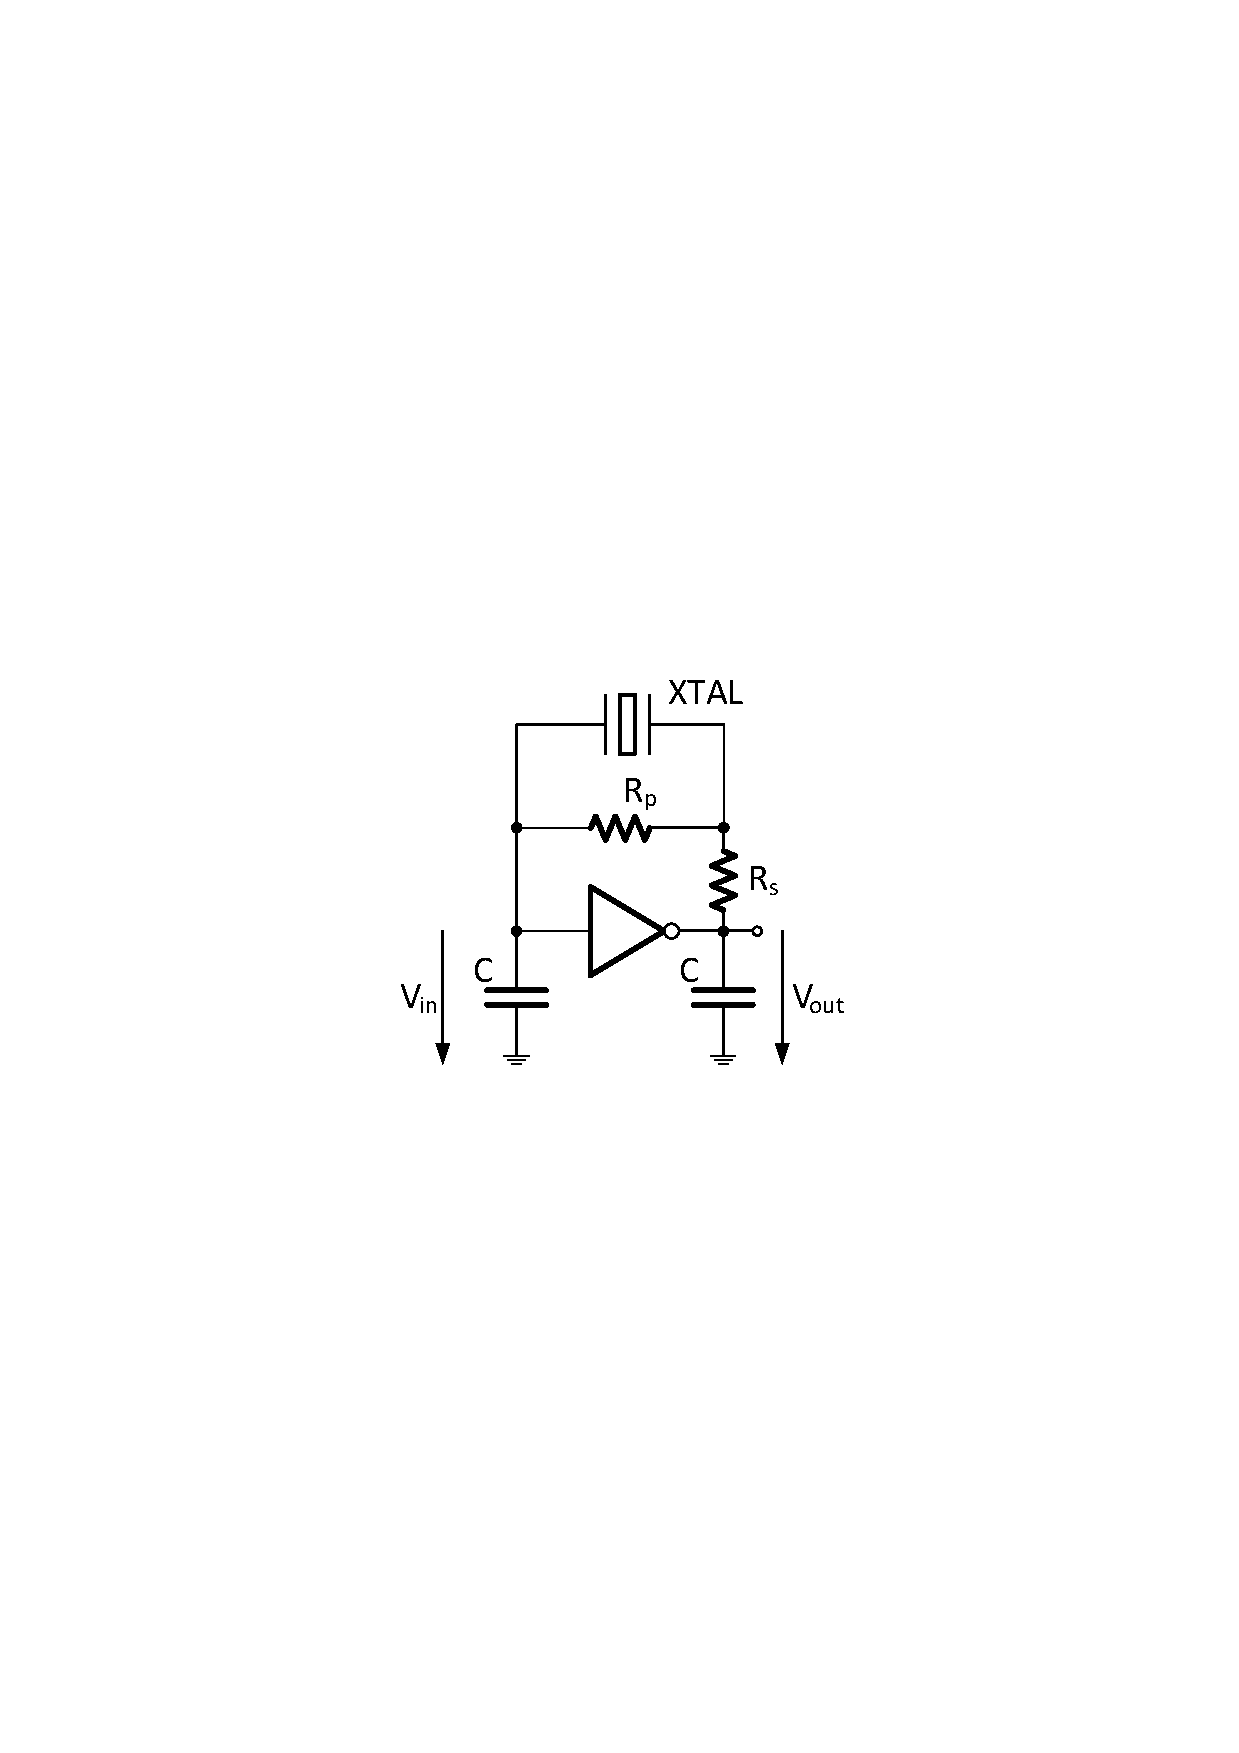
\includegraphics[width=6cm]{./Figures/Chap6_Horloges/Osc_XTAL_1.pdf}
  \caption{Schéma de l'oscillateur à quartz}
        \label{fig:Osc_XTAL_1}
    \end{minipage}%
    \begin{minipage}{0.5\textwidth}
        \centering
        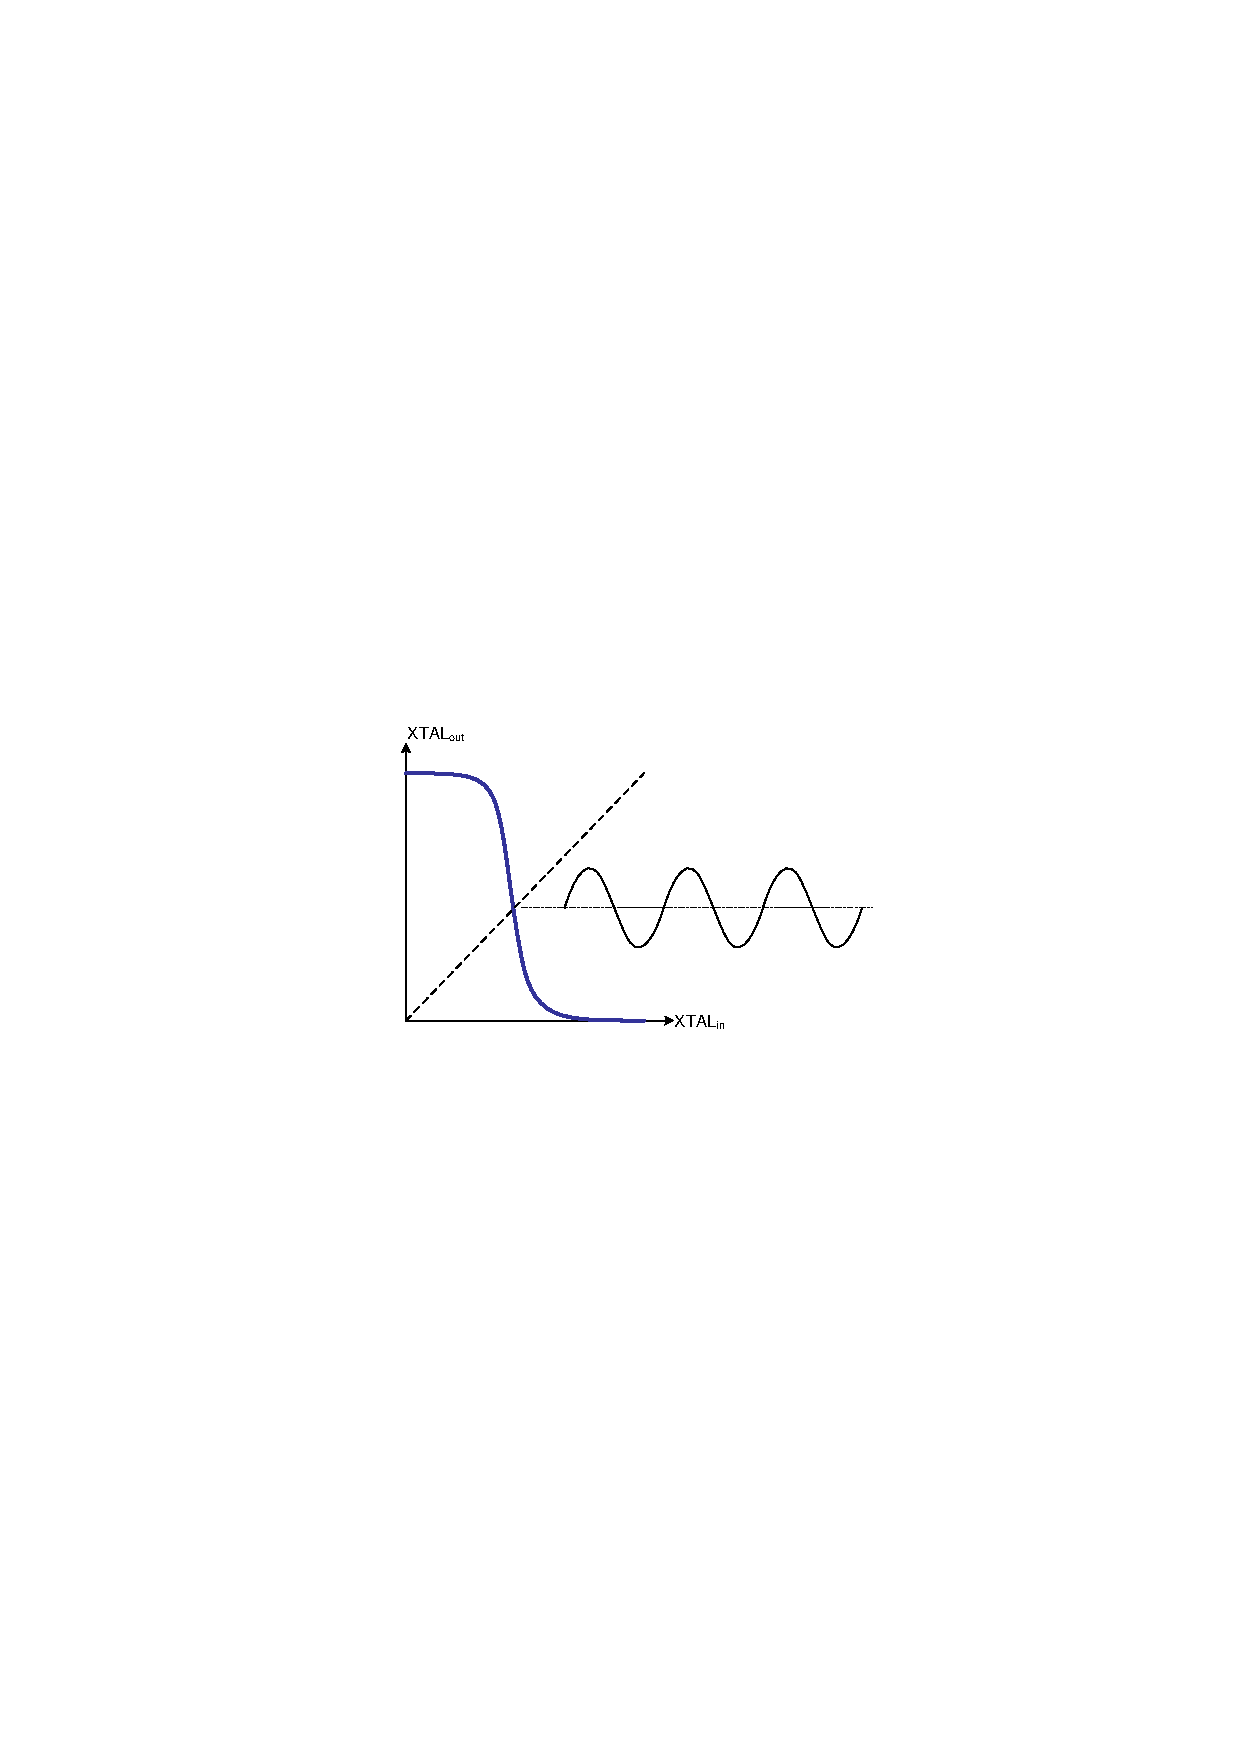
\includegraphics[width=6cm]{./Figures/Chap6_Horloges/XTAL_Pol.pdf}
        \caption{Polarisation de l'inverseur}
        \label{fig:XTAL_Pol}
    \end{minipage}
\end{figure}

Dans ce circuit, la résistance $R{p}$ a une grande valeur et ne sert qu'à polariser l'inverseur logique à son point de repos donnant le gain maximal. Ainsi connecté, l'inverseur maintien le résonateur en oscillation (figure \ref{fig:XTAL_Pol}). Le signal de sortie de l'inverseur est ensuite transformé en un signal carré qui constitue l'horloge de base pour le reste du circuit.

Une variante du résonateur à quartz est le résonateur céramique. Son fonctionnement est similaire à celui du quartz. Il se justifie pour son coût moindre, au prix de performances moindres.

\subsection{Critères de performance des oscillateurs}
Un oscillateur est caractérisé par:
\begin{itemize}[label=\textbullet,font=\small]
\item sa fréquence;
\item la précision de la fréquence;
\item la stabilité instantanée de la fréquence, qui est liée au facteur de qualité;
\item la stabilité de la fréquence dans le temps.
\end{itemize}

\subsubsection*{Fréquence}
Dans un oscillateur RC, la fréquence est peu précise car elle dépend de composants dont les valeurs sont peu précises. Dans un oscillateur à résonateur, la fréquence est essentiellement déterminée par le résonateur. Sa fréquence de résonance a une erreur relative, spécifiée en \textit{ppm}, ou \textit{part par million}. Un cristal de qualité moyenne a une erreur de fréquence de 100 ppm, soit 0,001\%.

\subsubsection*{Facteur de qualité}
Le facteur de qualité du signal est défini par $Q=\frac{f_{c}}{BW}$.
Si Q est grand, la bande passante est petite par rapport à la fréquence centrale de l'oscillation et donc la stabilité en fréquence est grande.

\subsubsection*{Stabilité}
La stabilité en fréquence d'un résonateur est aussi donnée en ppm.
La fréquence suit les dérives des composants. On distingue trois types de dérives :
\begin{itemize}[label=\textbullet,font=\small]
\item le vieillissement des composants, de l'ordre de 5 à 50 ppm;
\item l'effet des variations de température, de l'ordre de 20 à 200 ppm;
\item l'effet des variations d'humidité, en général inférieure à 10 ppm.
\end{itemize}

Ces trois effets sont liés à la nature mécanique du résonateur. Le vieillissement peut être associé au relâchement de tensions mécaniques internes au cours du temps. La température modifie les dimensions physiques du résonateur à cause de la dilatation. L'humidité diffuse dans le matériau lui-même.

\section{Multiplicateur de fréquence}
Un multiplicateur de fréquence contient deux fonctions de base :
\begin{itemize}[label=\textbullet,font=\small]
\item génération "libre" d'un signal à une fréquence proche de la fréquence visée;
\item asservissement de la fréquence obtenue à une fréquence de référence
\end{itemize}

\subsection{Principe de fonctionnement} 
\subsubsection*{Boucle ouverte}
Dans la version la plus simple du multiplicateur de fréquence, le facteur de multiplication est un nombre entier. Le signal de sortie est généré "librement" par un oscillateur contrôlé en tension (VCO, ou \textit{Voltage Controlled Oscillator }). Ce contrôle est nécessaire pour permettre l'asservissement. 
Le signal généré ayant une fréquence multiple de la fréquence de référence, il est divisé par un facteur N pour pouvoir être comparé avec cette dernière (figure \ref{fig:FLL_BO}).

\begin{figure}[htb]
  \centering
  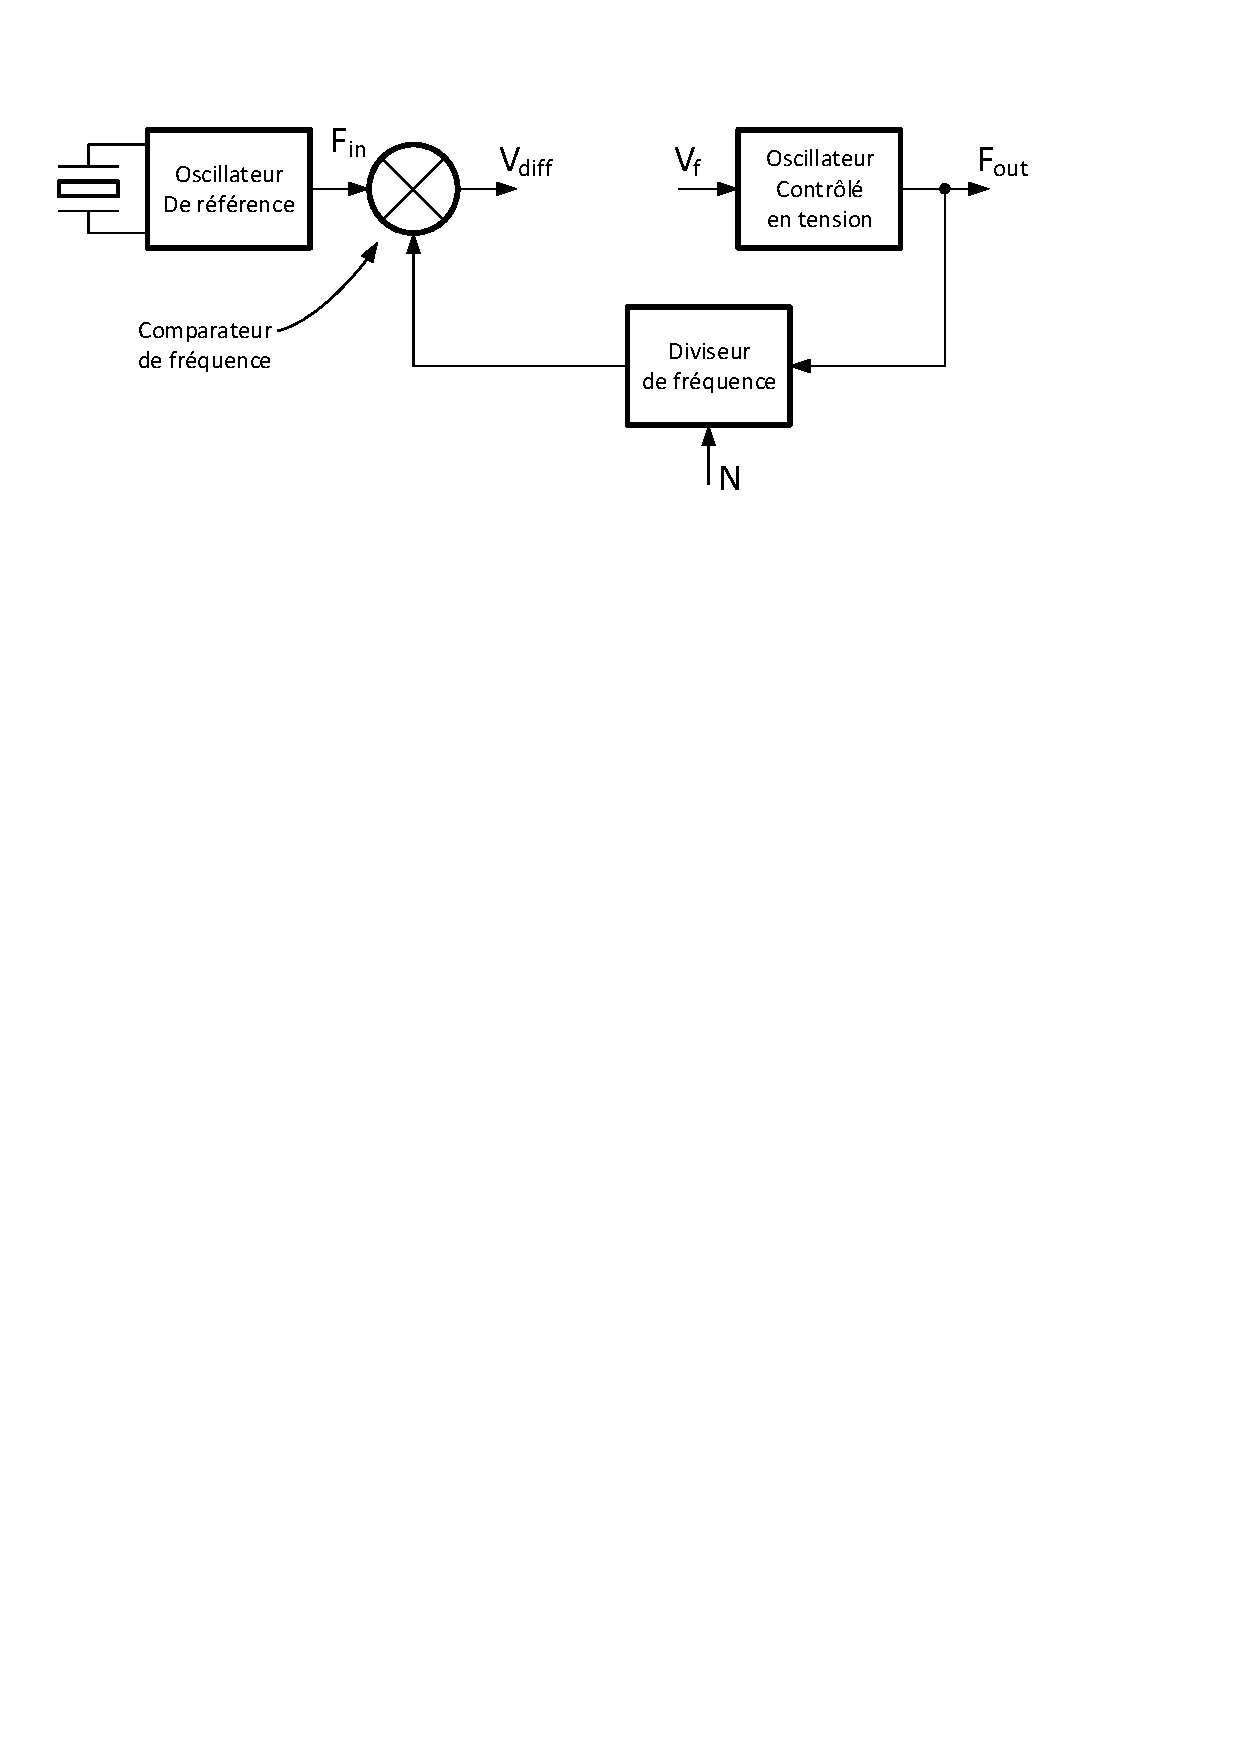
\includegraphics [angle=0, width=11cm]{./Figures/Chap6_Horloges/FLL_BO.pdf}
  \rule{35em}{0.5pt}
  \caption{Multiplicateur de fréquence - Boucle ouverte}
  \label{fig:FLL_BO}
\end{figure}

\subsubsection*{Boucle fermée}
Le comparateur de fréquence produit une tension proportionnelle à la différence des fréquences. Si la fréquence de référence est supérieure (resp. inférieure) à la fréquence de sortie divisée par N, alors la tension appliquée au VCO doit être réduite (resp. augmentée). Pour que cette tension soit stable, un filtre passe-bas est inséré entre la sortie du comparateur de fréquence et l'entrée du VCO (figure \ref{fig:FLL_BF}).\\
La fréquence du signal de sortie est : $F_{out}=N.F_{in}$

\begin{figure}[htb]
  \centering
  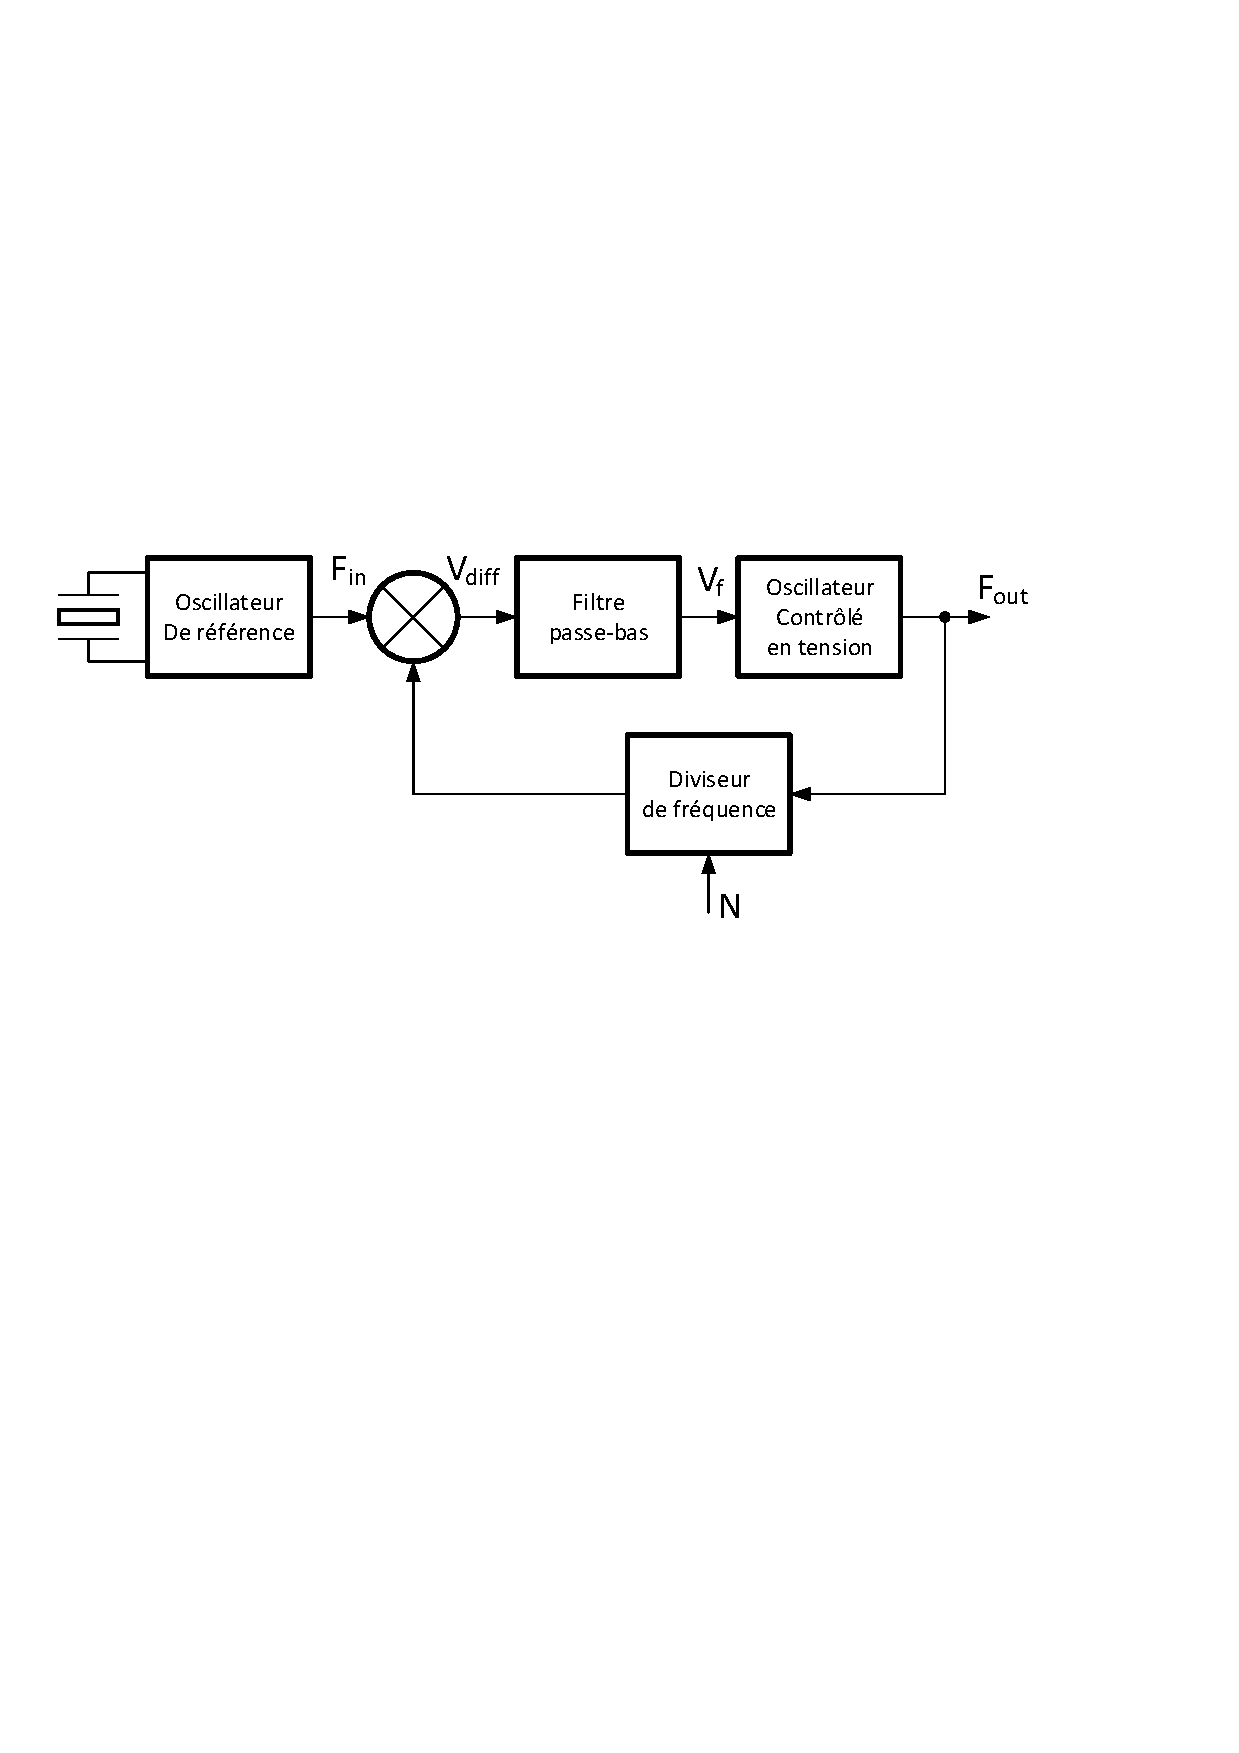
\includegraphics [angle=0, width=11cm]{./Figures/Chap6_Horloges/FLL_BF.pdf}
  \rule{35em}{0.5pt}
  \caption{Multiplicateur de fréquence - Boucle fermée}
  \label{fig:FLL_BF}
\end{figure}

\subsubsection*{Version embarquée}
Pour permettre un facteur de multiplication non-entier, il suffit d'ajouter un second diviseur de fréquence avant le comparateur de fréquence (figure \ref{fig:FLL_Frac}).

\begin{figure}[htb]
  \centering
  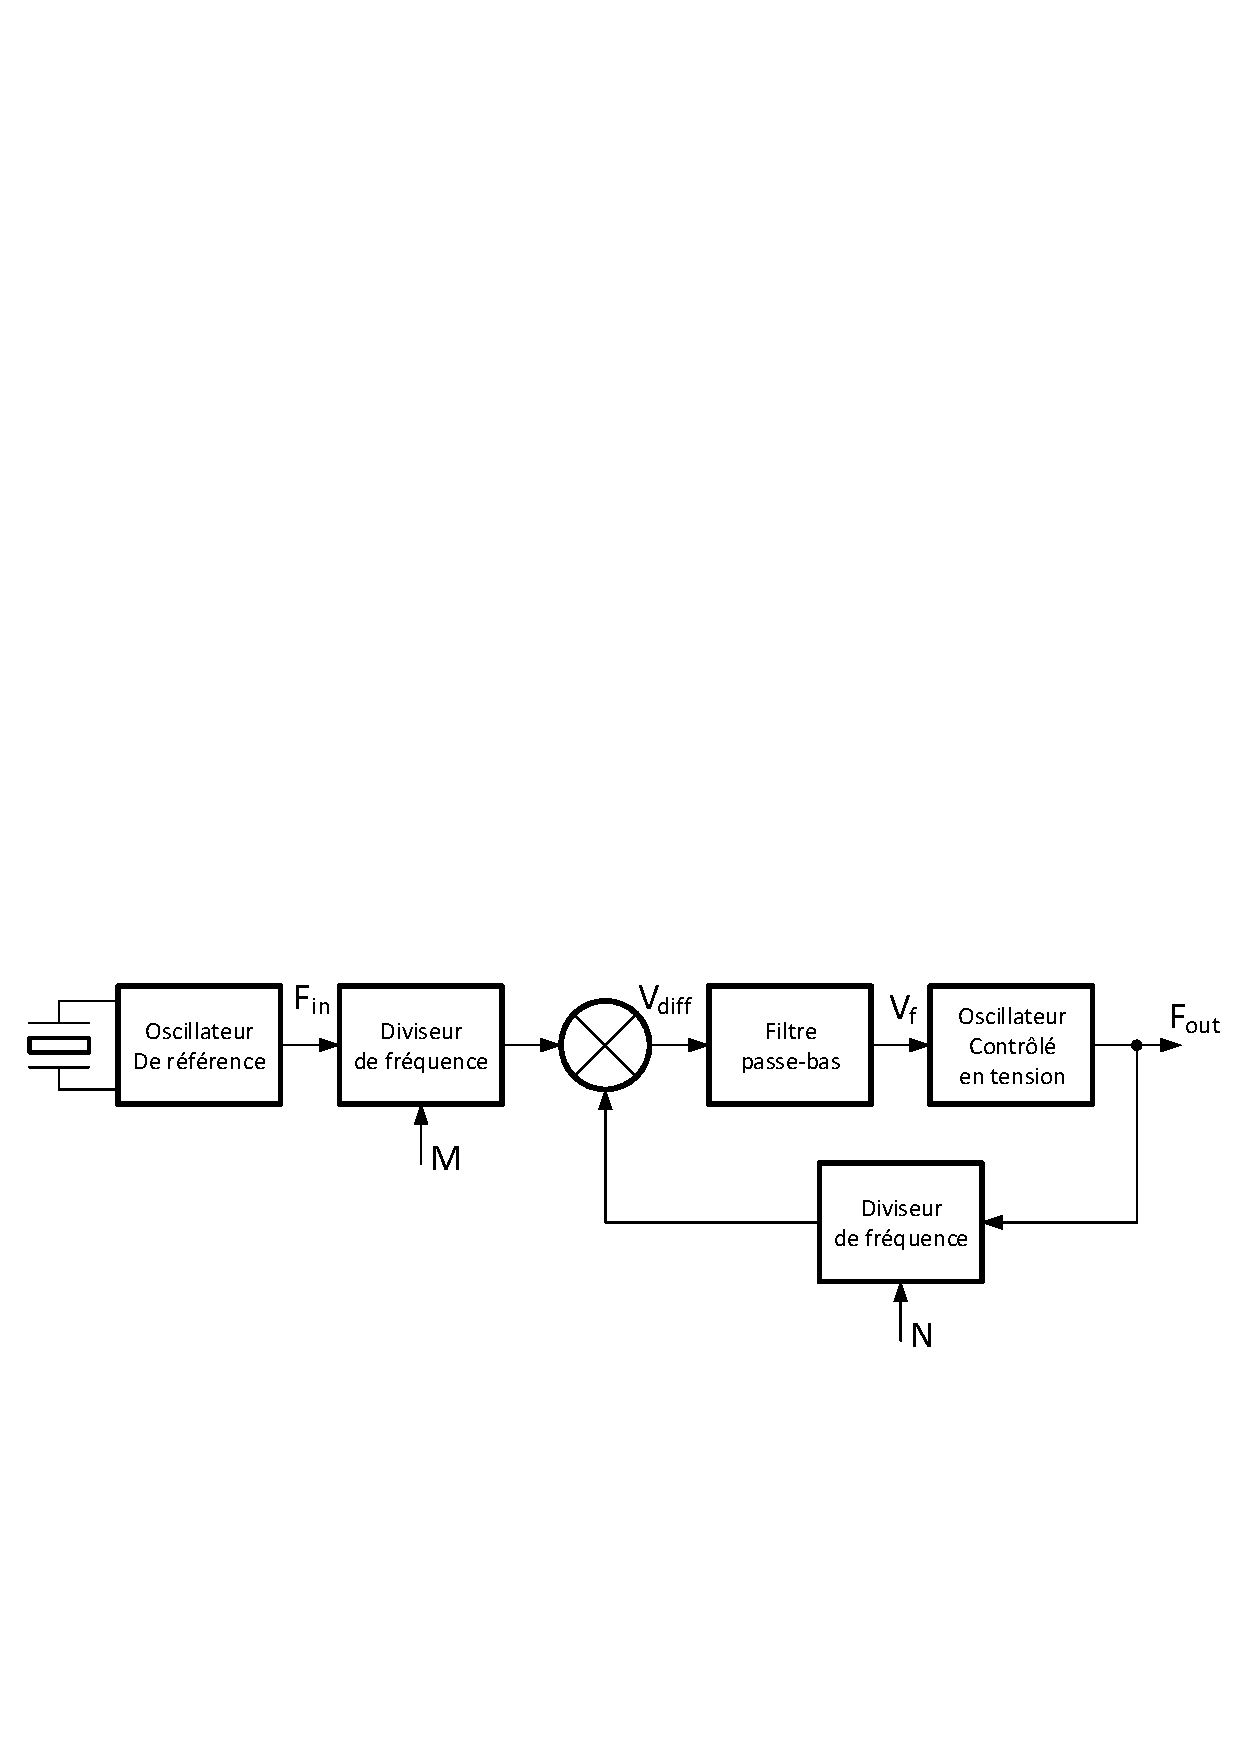
\includegraphics [angle=0, width=14cm]{./Figures/Chap6_Horloges/FLL_Frac.pdf}
  \rule{35em}{0.5pt}
  \caption{Multiplicateur de fréquence à facteur fractionnaire}
  \label{fig:FLL_Frac}
\end{figure}

La boucle de régulation tend à obtenir :\begin{LARGE} $\frac{F_{in}}{M}=\frac{F_{out}}{N}$ \end{LARGE}\\

La fréquence du signal de sortie est donc :\begin{LARGE} $F_{out}=\frac{N}{M}.F_{in}$\end{LARGE}\\

En pratique, le comparateur de fréquence et le filtre passe-bas sont réalisés au moyen d'un intégrateur numérique, qui consiste en un compteur/décompteur. Durant un intervalle de temps défini, celui-ci s'incrémente sur les impulsions du signal de référence et se décrémente sur les impulsions du signal de sortie. A la fin de l'intervalle de temps, on sait si le VCO doit augmenter ou réduire la fréquence du signal de sortie. Une conséquence importante est que la fréquence moyenne du signal de sortie est stable, mais la fréquence instantanée varie en dents de scie.

\pagebreak
\section{Cas du MSP430} 
La figure \ref{fig:UCS_Blocs} est un schéma synoptique du circuit d'horloge, appelé UCS pour \textit{Unified Clock System}. Ceci est valable pour les microcontrôleurs de la famille MSP430F5xxx.\\
Cinq sources de fréquence sont disponibles:
\begin{itemize}[label=\textbullet,font=\small]
\item VLOCLK: oscillateur interne basse fréquence à très basse consommation, dont la fréquence est d'environ 10 kHz
\item REFOCLK: oscillateur interne calibré à environ 32768 Hz;
\item XT1CLK: oscillateur à large gamme de fréquence, pouvant être connecté à un résonateur à quartz ou céramique 32768 Hz, ou une source externe de 4 MHz à 32 MHz;
\item XT2CLK: oscillateur haute fréquence (en option), pouvant être connecté à un résonateur à quartz ou céramique ou une source externe;
\item DCOCLK : horloge obtenue par multiplication de l'une des 4 sources précédentes.
\end{itemize}

\bigskip 
A partir de ces 5 sources, qui peuvent être activées ou désactivées chacune individuellement, le circuit UCS produit 3 signaux d'horloge pour le CPU et les différents périphériques du microcontrôleur:
\begin{itemize}[label=\textbullet,font=\small]
\item ACLK (Auxiliary Clock) est plutôt réservé aux périphériques à basse consommation ou se contentant d'une horloge à basse fréquence, comme les timers. Toutefois, ACLK peut être connecté à n'importe laquelle des 5 sources de fréquence.
\item SMCLK (Subsystem Master Clock) est disponible pour les périphériques;
\item MCLK (Master Clock) est l'horloge du CPU;
\end{itemize}

\begin{figure}[htb]
  \centering
  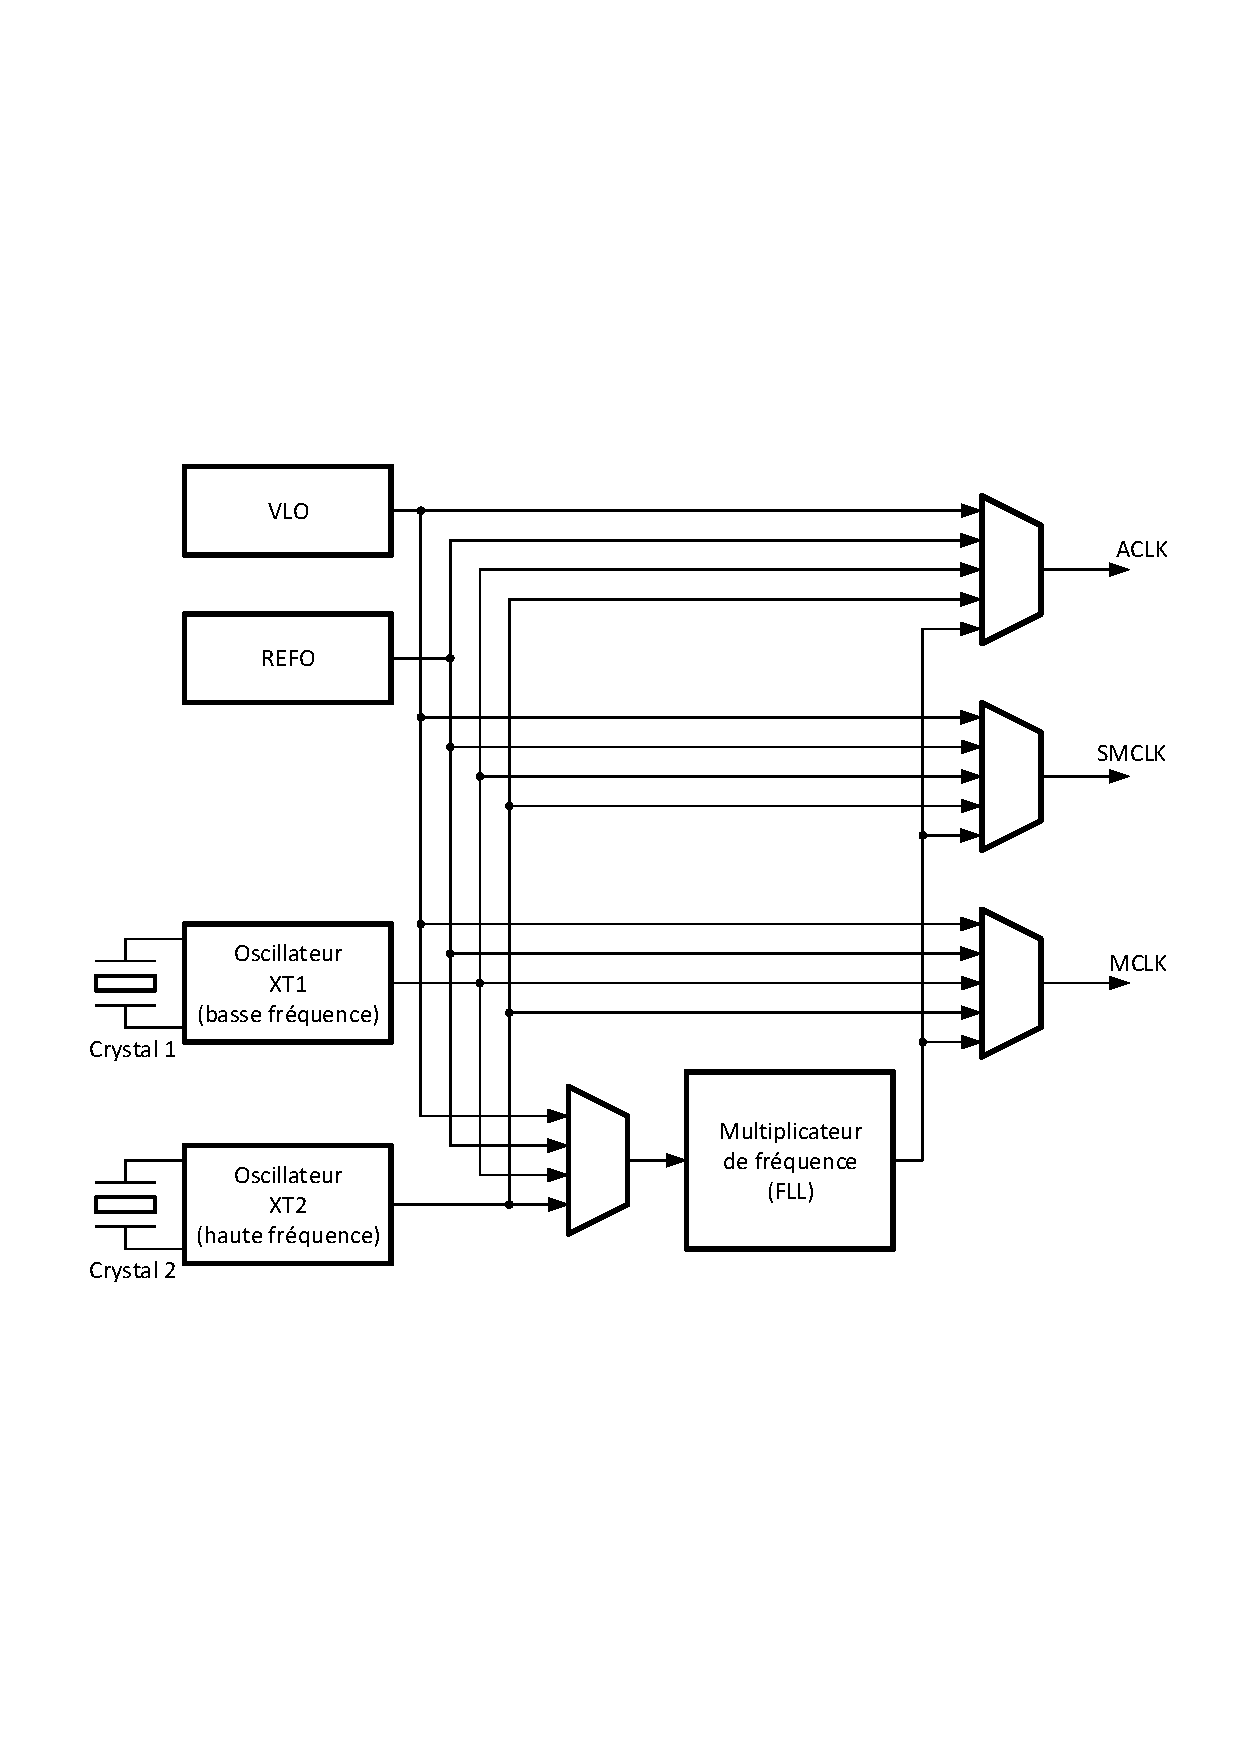
\includegraphics [angle=0, width=14cm]{./Figures/Chap6_Horloges/UCS_Blocs.pdf}
  \rule{35em}{0.5pt}
  \caption{Schéma synoptique du circuit d'horloge du MSP430}
  \label{fig:UCS_Blocs}
\end{figure}

\subsection{Frequency Locked Loop}
Le multiplicateur de fréquence est nommé \textit{Frequency Locked Loop}. Son schéma est donné à la figure \ref{fig:UCS_FLL}. On retrouve les éléments vus au chapitre \ref{Multiplicateur de fréquence}:
\begin{itemize}[label=\textbullet,font=\small]
\item 10-bit Frequency integrator : le comparateur de fréquence
\item DCO : le VCO
\item Prescaler et Divider/(N+1) : le diviseur de $F_{out}$
\item Divider (/1/2/4/8/12/16) : le diviseur de $F_{ref}$
\end{itemize}

La fréquence du signal de sortie DCOCLK est donnée par :
\begin{tabbing}
\begin{Large}
\qquad $F_{DCOCLK}=F_{FLLREFCLK}.\frac{(FLLN+1).(FLLD)}{FLLREFDIV}$
\end{Large}
\end{tabbing}
\bigskip
L'élément \textit{DC Generator} génère un courant de polarisation pour le VCO. Il permet aussi de sélectionner la gamme de fréquences que peut générer le VCO. Ces fréquences sont comprises dans un intervalle de quelques dizaines de MHz, mais le VCO ne peut pas toutes les générer simultanément. La gamme de fréquence est donc déterminée par le \textit{DC Generator}. Les différentes gammes dépendent du modèle de microcontrôleur.

\begin{figure}[htb]
  \centering
  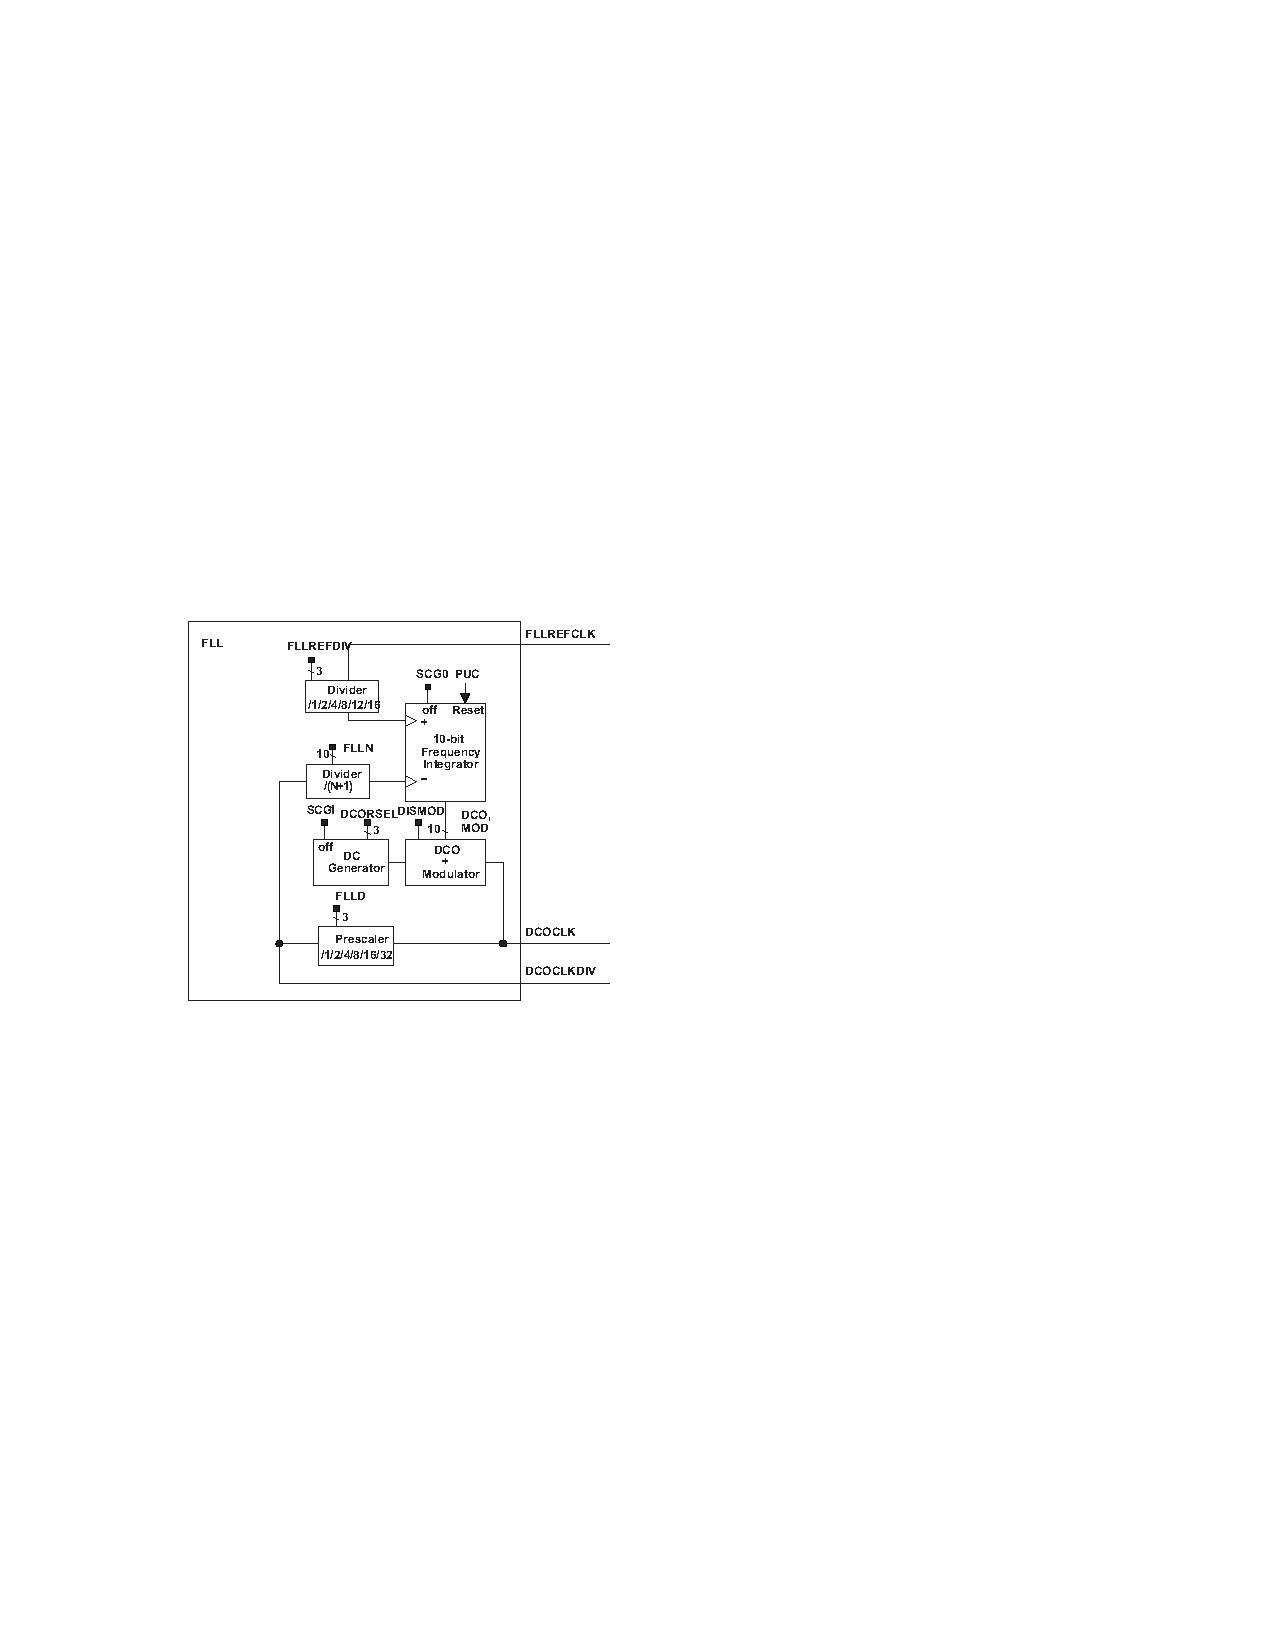
\includegraphics [angle=0, width=14cm]{./Figures/Chap6_Horloges/UCS_FLL.pdf}
  \rule{35em}{0.5pt}
  \caption{Schéma du multiplicateur de fréquence}
  \label{fig:UCS_FLL}
\end{figure}

A titre d'exemple, la figure \ref{fig:FLL_Gammes} donne les gammes de fréquence que le MSP430F5529 peut générer. Si le paramètre DCORSEL (DCO Range Select) est mal configuré, la fréquence visée sera trop excentrée dans la gamme sélectionnée, voire hors de la gamme, et la boucle de régulation de la FLL ne pourra faire son travail correctement.

\begin{figure}[!htb]
  \centering
  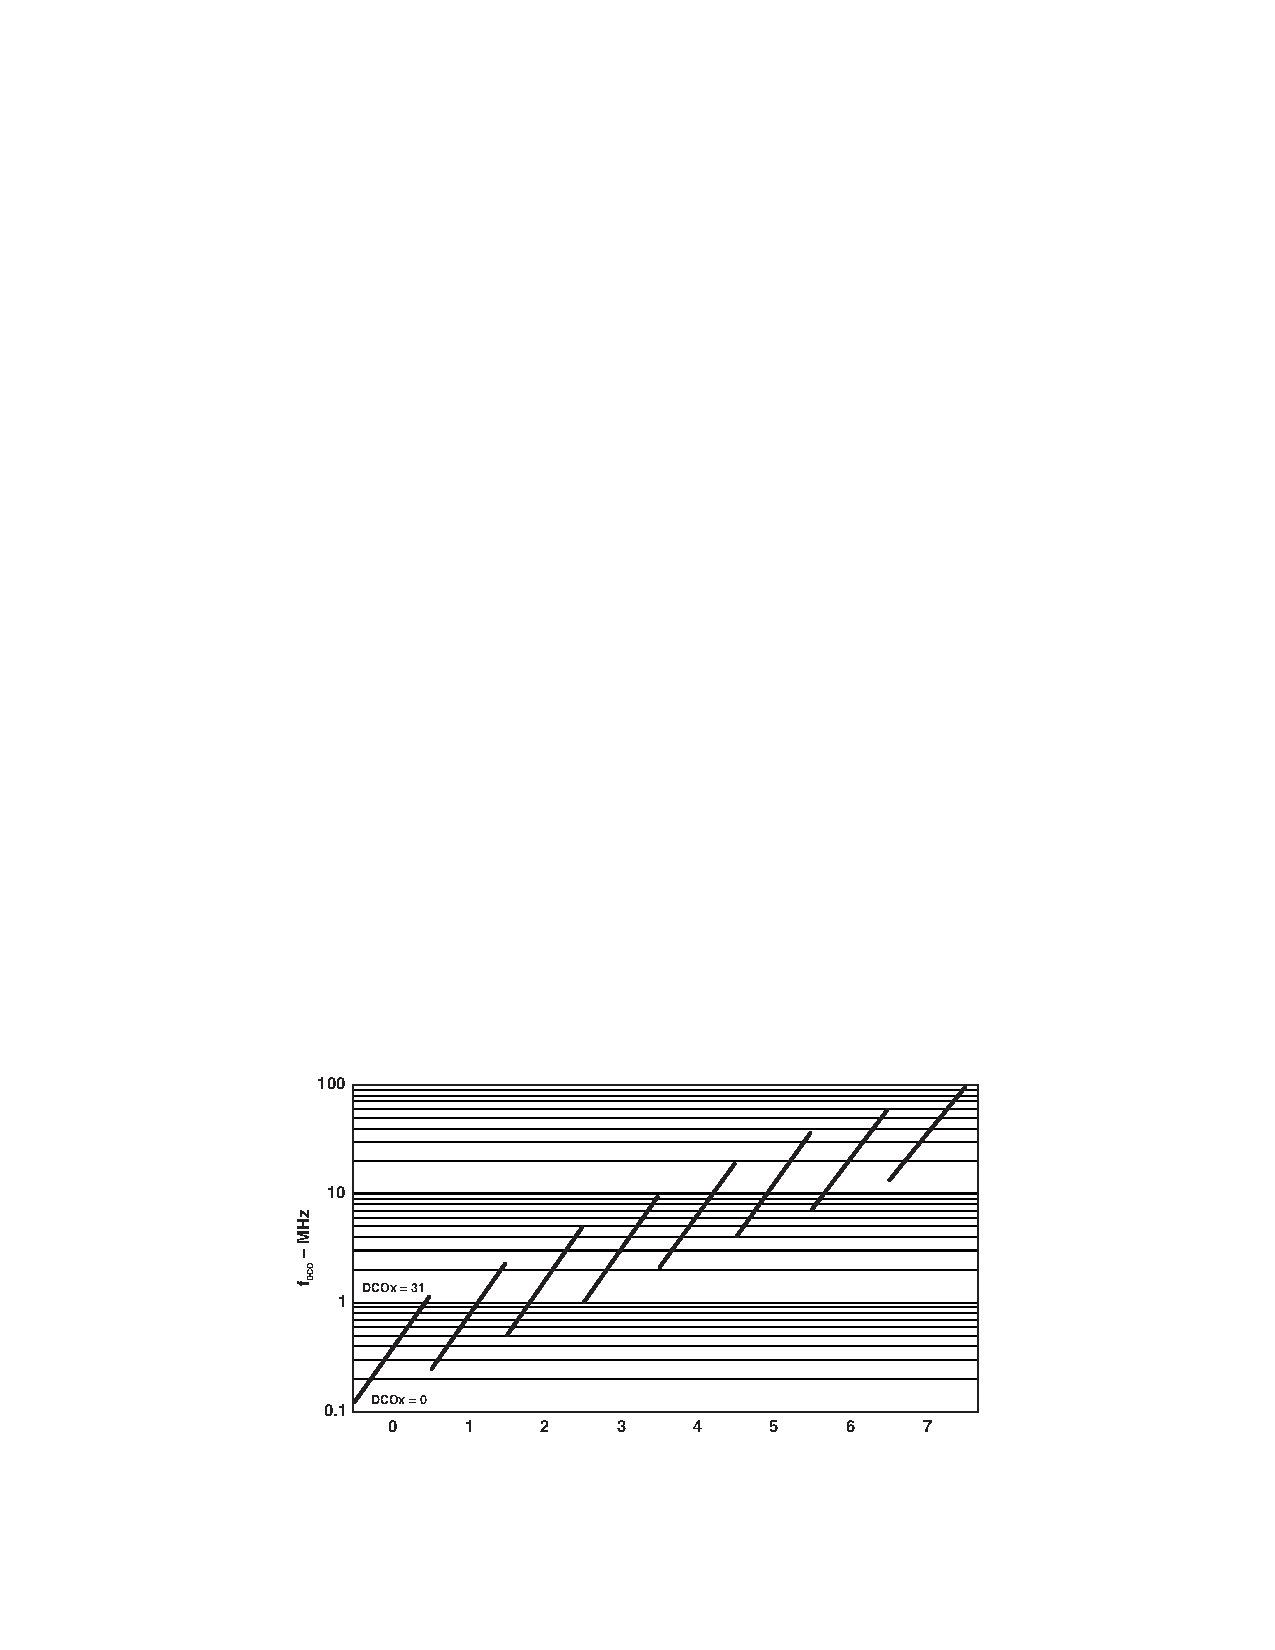
\includegraphics [angle=0, width=14cm]{./Figures/Chap6_Horloges/FLL_Gammes.pdf}
  \rule{35em}{0.5pt}
  \caption{Gammes de fréquence du MSP430F5529}
  \label{fig:FLL_Gammes}
\end{figure}



\subsubsection*{Exemple}
On souhaite générer une fréquence de 3,2768 MHz à partir d'une horloge de 32768 Hz. On peut choisir DCORSEL = 2,3 ou 4. La valeur 2 est la meilleure car la gamme correspondante est la mieux centrée autour de 3,2768 MHz.
Le facteur de multiplication vaut 100. Il peut être obtenu avec :
\begin{itemize}[label=\textbullet,font=\small]
\item $FLLREFDIV = 1$;
\item $FLLD = 2$;
\item $FLLN = 49$.
\end{itemize}


\subsection{Configuration du circuit UCS}
Le schéma détaillé du circuit UCS est donné à la figure \ref{fig:UCS_Schema}. En plus des 5 sources de fréquence principales décrites précédemment, une $6^{eme}$ source est visible: il s'agit de la sortie du \textit{prescaler}, elle est notée DCOCLKDIV. De plus, 2 autres signaux d'horloge sont visibles, en plus de ACLK, MCLK et SMCLK. Ce sont ACLK/n, qui est dérivée de ACLK par une division de fréquence et disponible sur une patte externe du microcontrôleur, et MODCLK qui sert pour certains périphériques spéciaux dont le convertisseur AD. Finalement, les horloges ACLK, MCLK et SMCLK peuvent subir une postdivision de fréquence par 1, 2, 4, 8, 12, 16, 32.

La configuration du circuit UCS demande donc de spécifier :
\begin{itemize}[label=\textbullet,font=\small]
\item la connection des 3 horloges (ACL, MCLK, SMCLK) avec les 6 sources de fréquence, y compris DCOCLKDIV. Ceci se fait par des champs appelés SELx dans les divers registres de configuration.
\item le facteur de prédivision des horloges ACLK, MCLK et SMCLK. Ceci se fait par des champs appelés DIVx dans les divers registres de configuration.
\item la configuration de la FLL si elle est utilisée. Ceci comprend:
\begin{itemize}[label=\textbullet,font=\footnotesize]
\item Détermination des facteurs FLLREFDIV, FLLN et FLLD, de façon à approcher au mieux la fréquence visée, à partir de la fréquence de référence;
\item Détermination du facteur DCORSEL.
\end{itemize}
\end{itemize}

\subsection{Registres de contrôle du circuit UCS}
Ils sont nommés UCSCTLx et sont au nombre de 10. En principe, on ne touche pas à UCSCTL0, qui contient des grandeurs internes au comparateur de fréquence. Les plus couramment utilisés sont :
\begin{itemize}[label=\textbullet,font=\small]
\item UCSCTL1: contient DCORSEL (figure \ref{fig:UCSCTL1} et table \ref{table:UCSCTL1});
\item UCSCTL2 et UCSCTL3 : configuration du multiplieur de fréquence FLL (figures \ref{fig:UCSCTL2} et \ref{fig:UCSCTL3} et tables \ref{table:UCSCTL2} et \ref{table:UCSCTL3}); 
\item UCSCTL4: connections de ACLK, MCLK et SMCLK (figure \ref{fig:UCSCTL4} et table \ref{table:UCSCTL4});
\item UCSCTL5: facteurs de prédivision de ACLK, MCLK et SMCLK (figure \ref{fig:UCSCTL5} et table \ref{table:UCSCTL5});
\end{itemize}
Les autres registres permettent de faire des réglages fins sur les oscillateurs XT1 et XT2.

\begin{figure}[H]
  \centering
  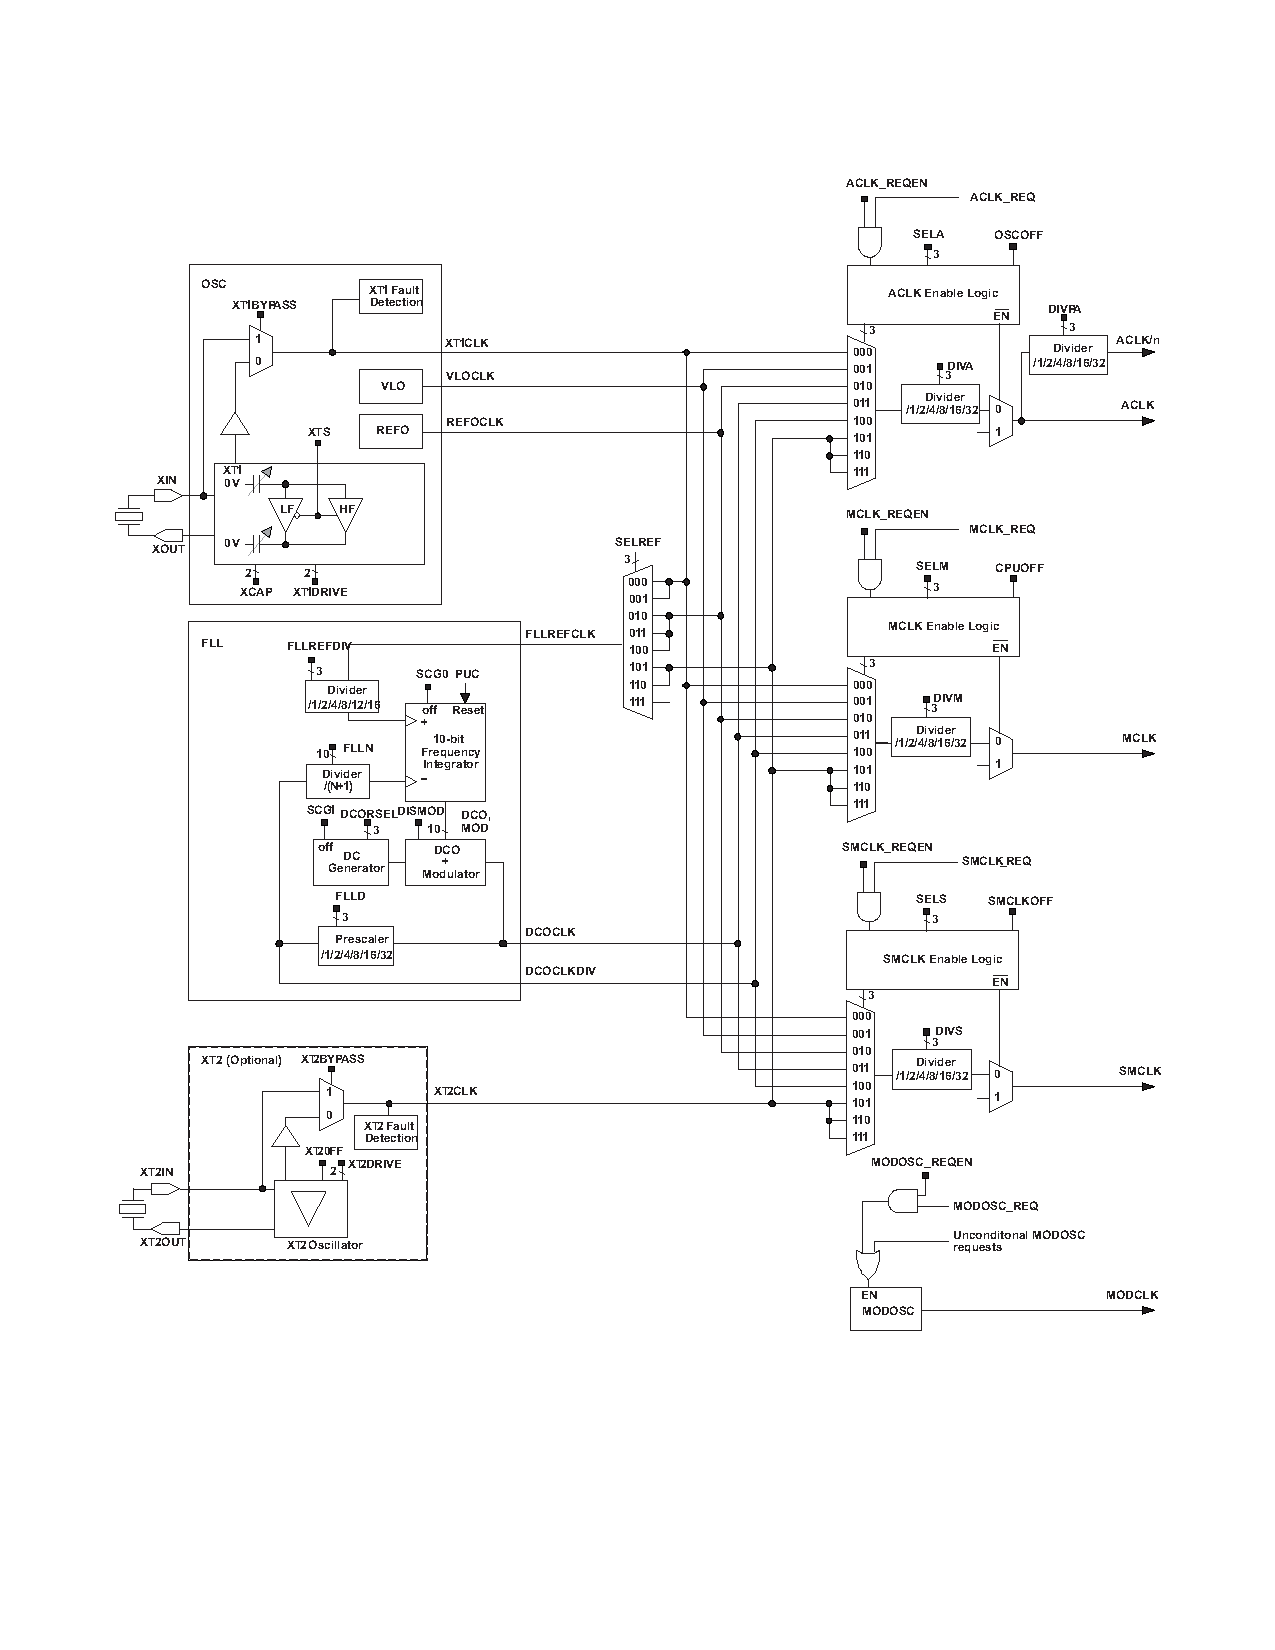
\includegraphics [angle=0, width=16cm]{./Figures/Chap6_Horloges/UCS_Schema.pdf}
  \rule{35em}{0.5pt}
  \caption{Schéma complet du circuit UCS}
  \label{fig:UCS_Schema}
\end{figure}

\pagebreak
\begin{figure}[H]
  \centering
  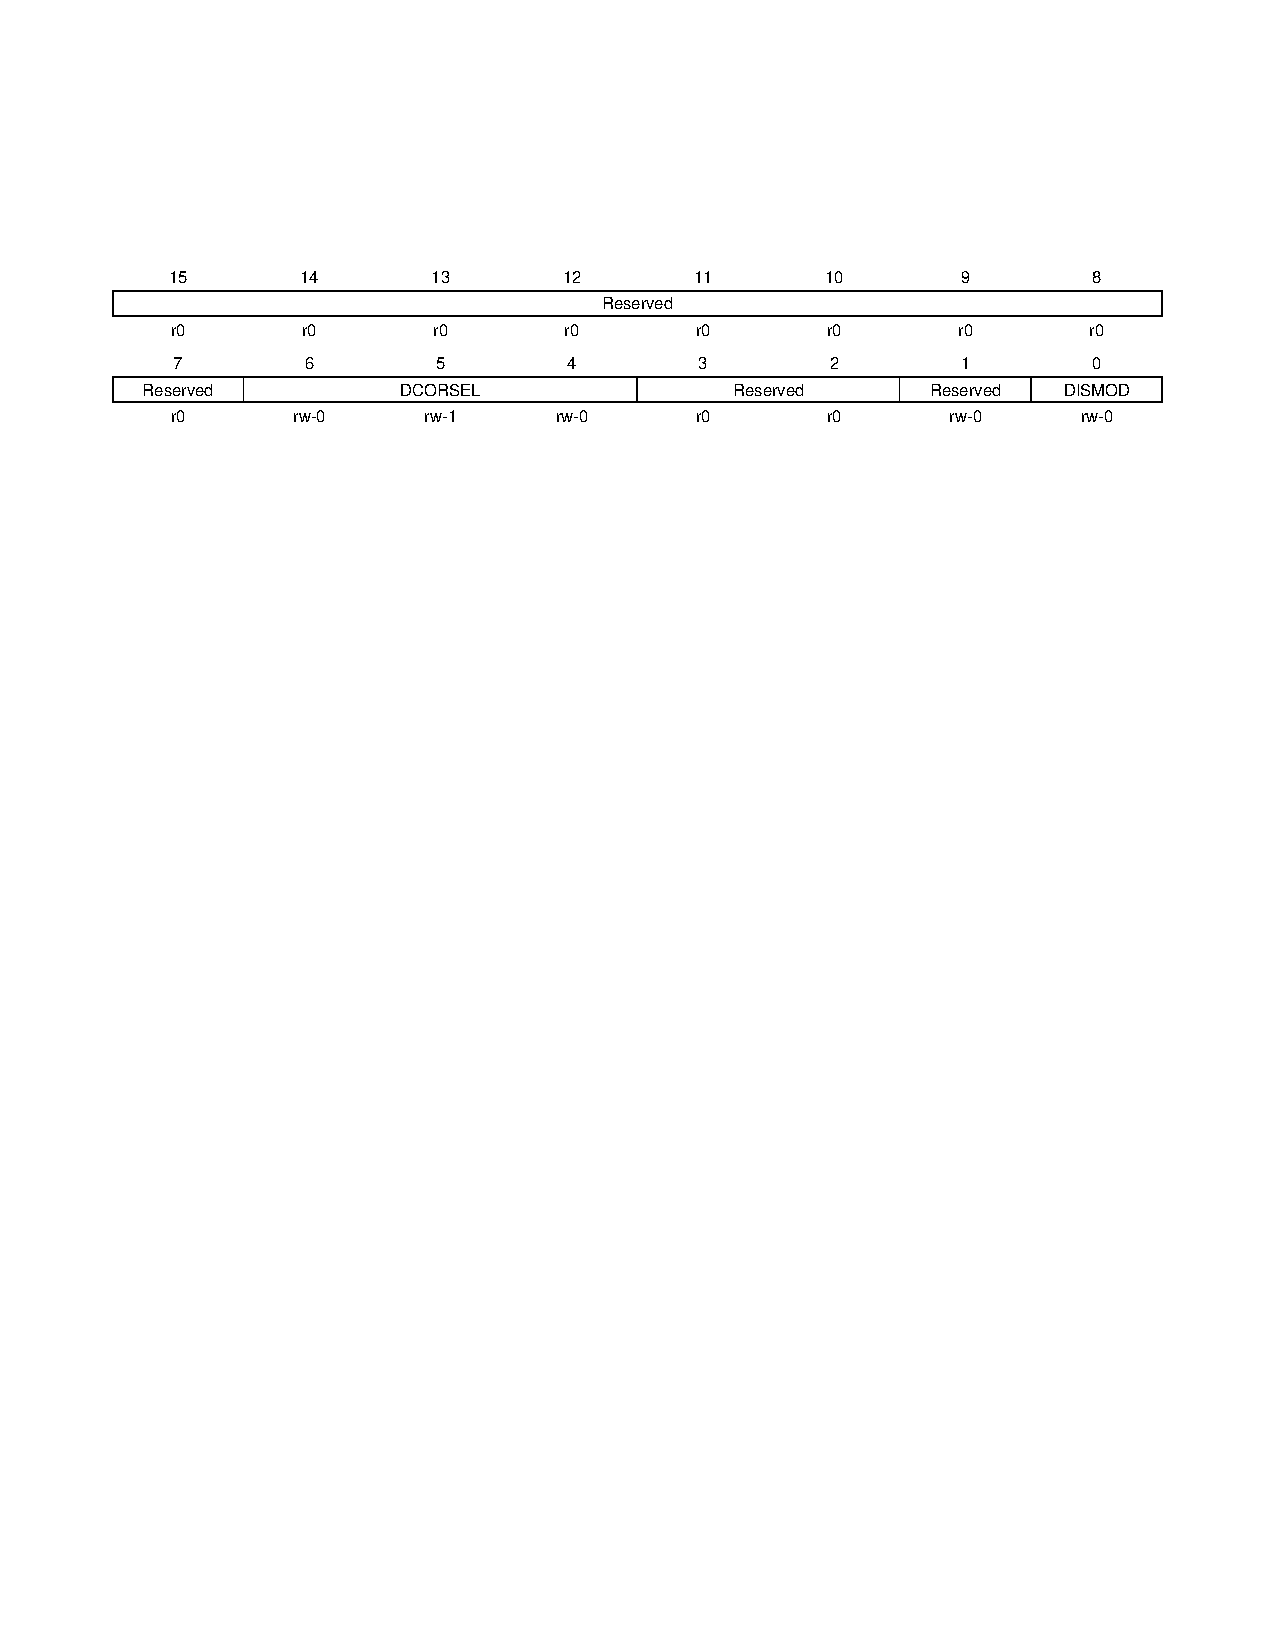
\includegraphics [angle=0, width=16cm]{./Figures/Chap6_Horloges/UCSCTL1.pdf}
  \rule{35em}{0.5pt}
  \caption{UCSCTL1}
  \label{fig:UCSCTL1}
\end{figure}

\begin{table}[H]
\centering 
\begin{tabular}{l l l l}
\hline\hline
Champ & & Valeur & Description \\ %[0.5ex]
\hline
DCORSEL & & & Sélection de la gamme (voir figure \ref{fig:FLL_Gammes})  \\
\hline
DISMOD & & - & Fonction liée au comportement interne du comparateur de fréquence \\
\hline
\end{tabular}
\caption{UCSCTL1}
\label{table:UCSCTL1}
\end{table}

\begin{figure}[H]
  \centering
  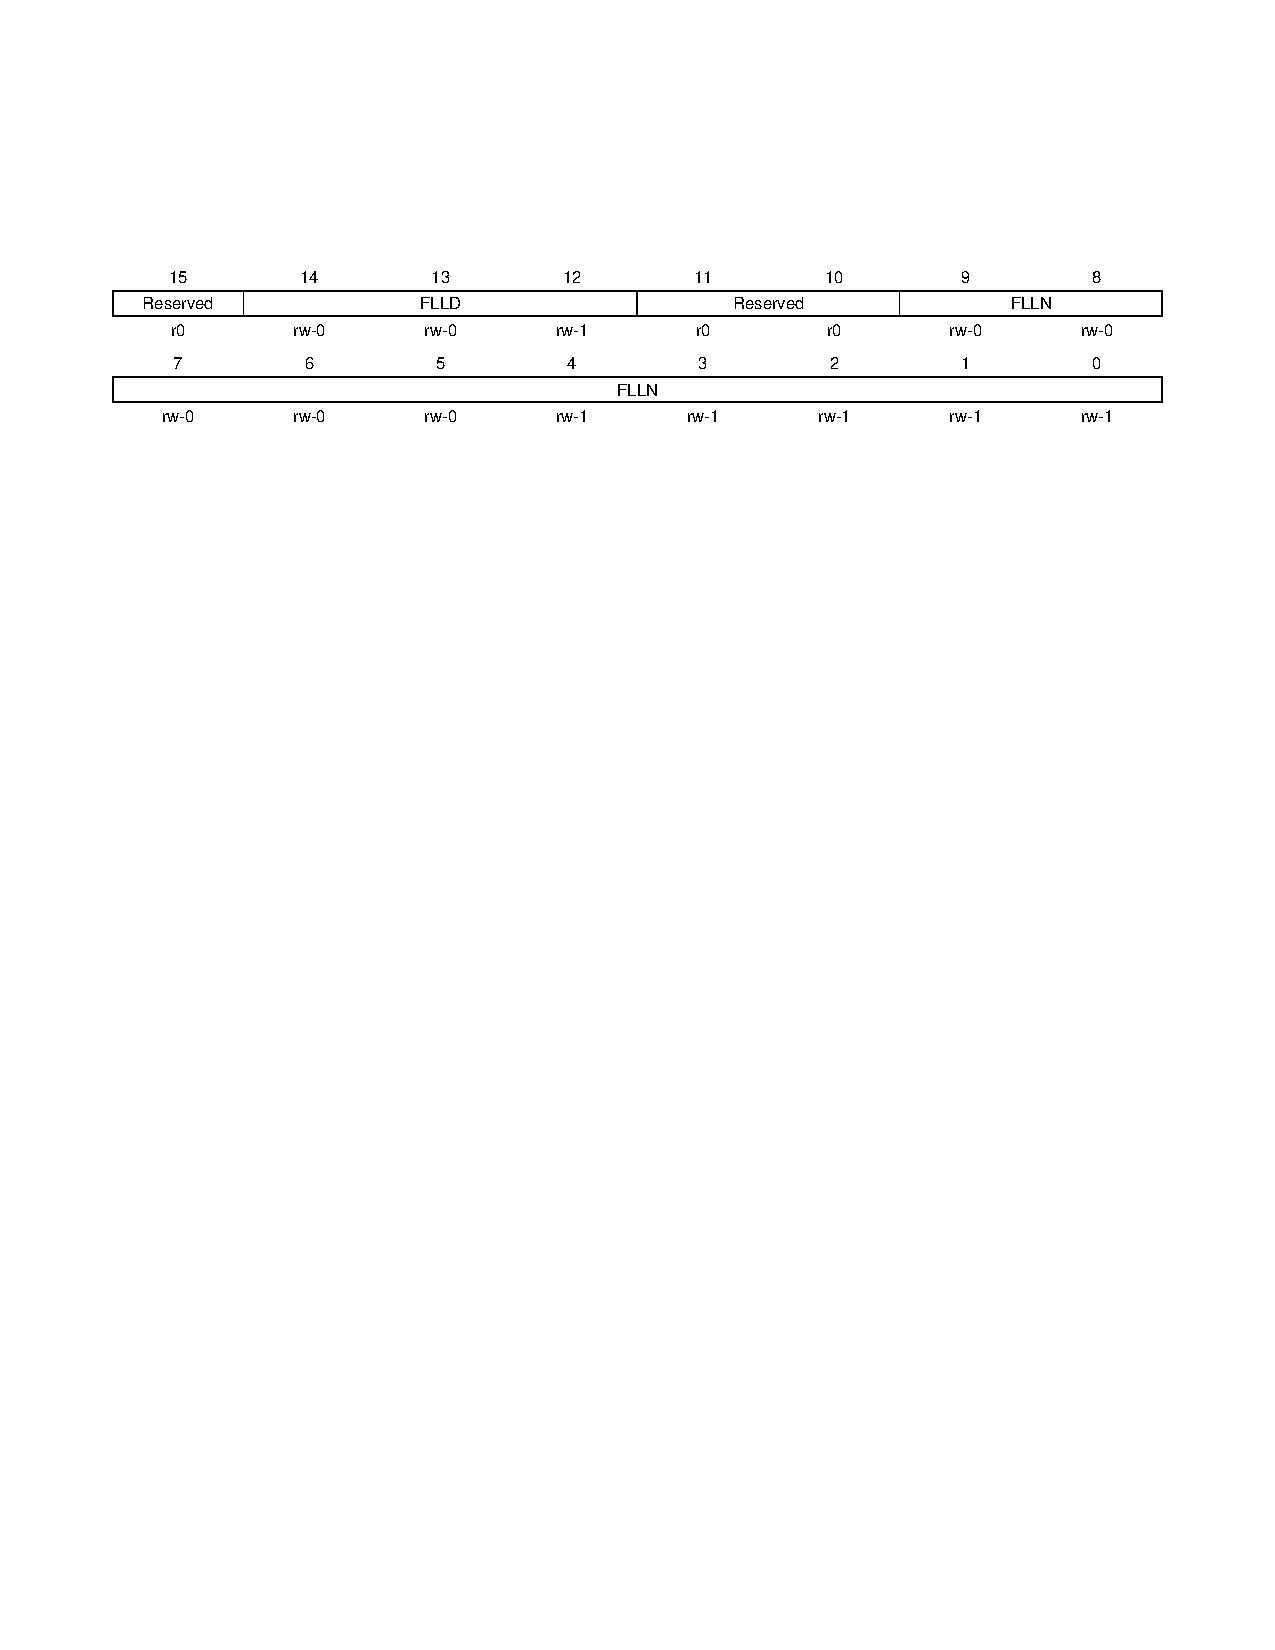
\includegraphics [angle=0, width=16cm]{./Figures/Chap6_Horloges/UCSCTL2.pdf}
  \rule{35em}{0.5pt}
  \caption{UCSCTL2}
  \label{fig:UCSCTL2}
\end{figure}

\begin{table}[H]
\centering 
\begin{tabular}{l l l l}
\hline\hline
Champ & & Valeur & Description \\ %[0.5ex]
\hline
FLLD & & & Facteur de multiplication ($F_{DCOCLK}=F_{FLLREFCLK}.\frac{(FLLN+1).(FLLD)}{FLLREFDIV}$)  \\
& & 000 & FLLD = 1 \\
& & 001 & FLLD = 2 \\
& & 010 & FLLD = 4 \\
& & 011 & FLLD = 8 \\
& & 100 & FLLD = 16 \\
& & 101 & FLLD = 32 \\
& & 110 & réservé \\
& & 111 & réservé \\
\hline
FLLN & & & Facteur de multiplication (voir chapitre {Frequency Locked Loop} \\
\hline
\end{tabular}
\caption{UCSCTL2}
\label{table:UCSCTL2}
\end{table}

\pagebreak
\begin{figure}[H]
  \centering
  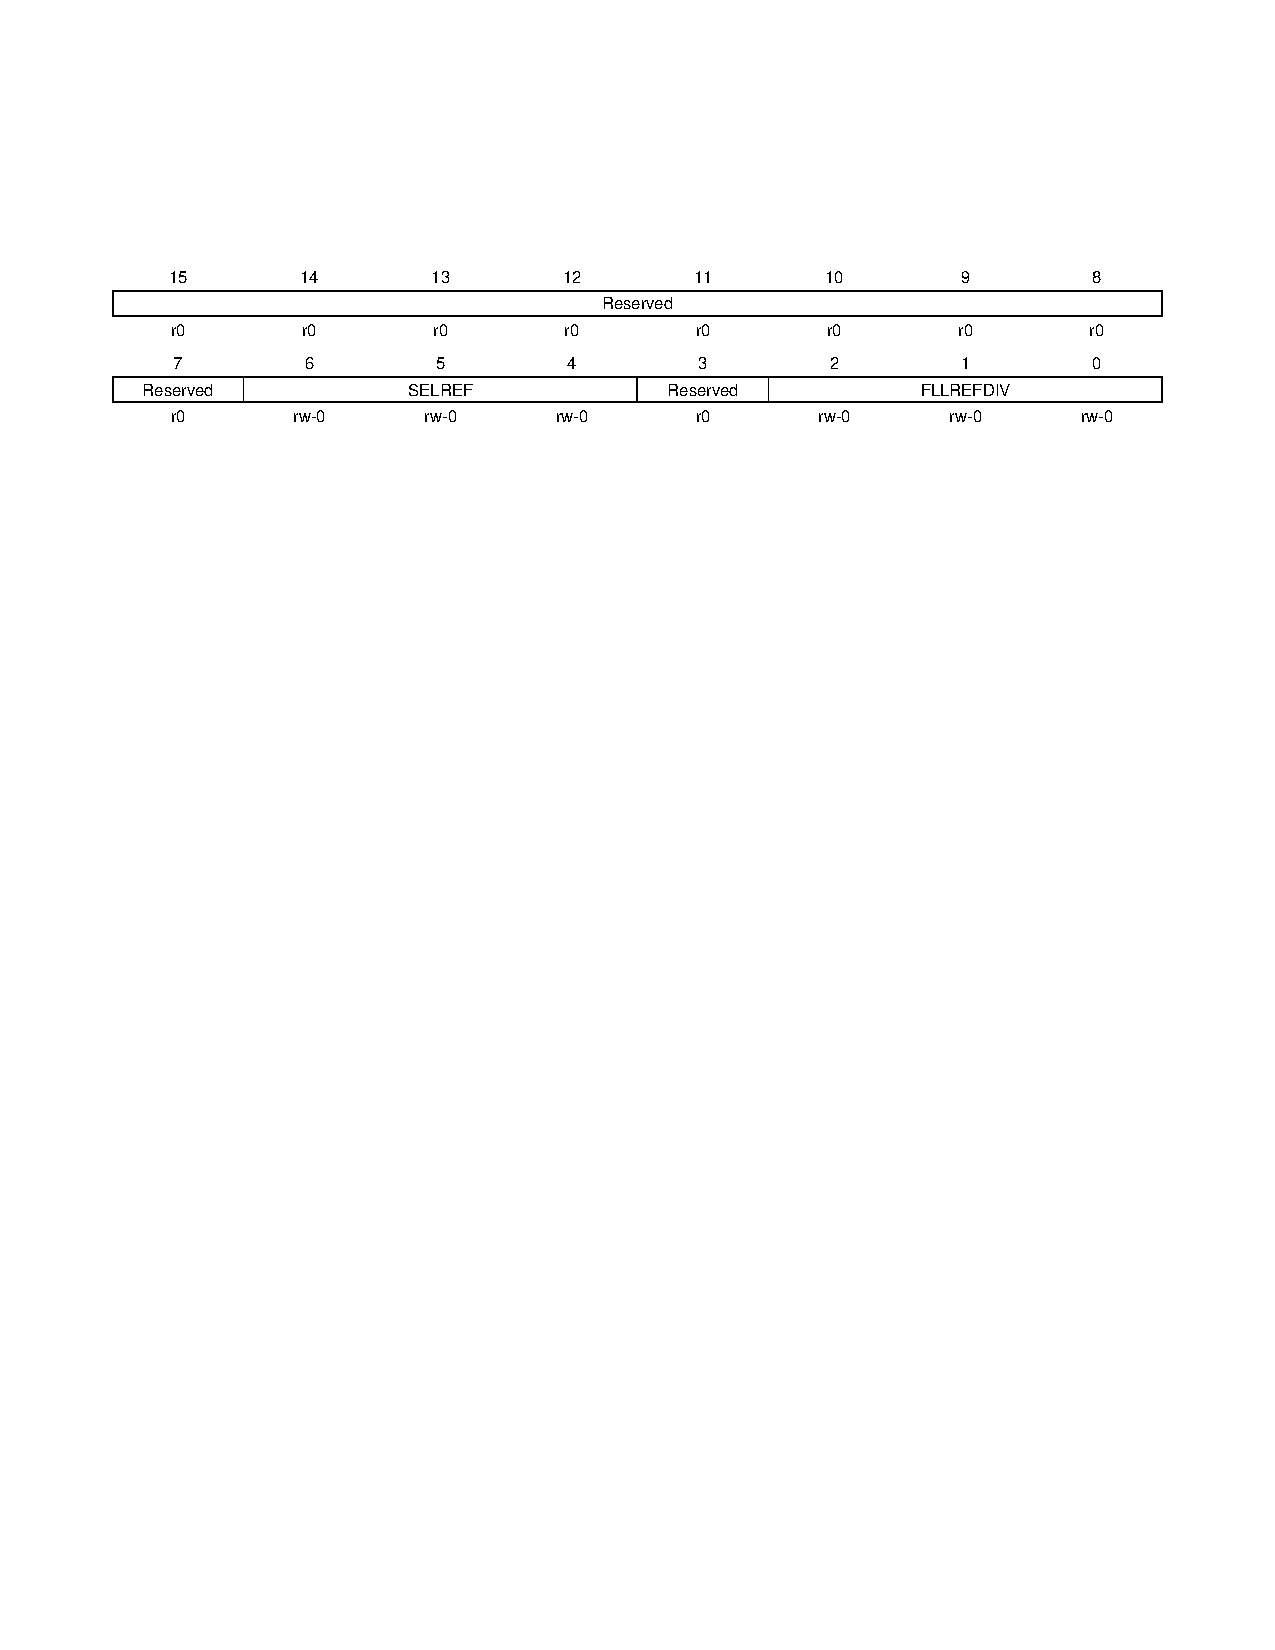
\includegraphics [angle=0, width=16cm]{./Figures/Chap6_Horloges/UCSCTL3.pdf}
  \rule{35em}{0.5pt}
  \caption{UCSCTL3}
  \label{fig:UCSCTL3}
\end{figure}

\begin{table}[H]
\centering 
\begin{tabular}{l l l l}
\hline\hline
Champ & & Valeur & Description \\ %[0.5ex]
\hline
SELREF & & & Sélection de la source de référence  \\
& & 000 & XT1CLK \\
& & 001 & réservé \\
& & 010 & REFOCLK \\
& & 011 & réservé \\
& & 100 & réservé \\
& & 101 & XT2CLK \\
& & 110 & réservé \\
& & 111 & réservé \\
\hline
FLLREFDIV & & & Prédivision de la référence ($F_{DCOCLK}=F_{FLLREFCLK}.\frac{(FLLN+1).(FLLD)}{FLLREFDIV}$) \\
& & 000 & FLLREFDIV = 1 \\
& & 001 & FLLREFDIV = 2 \\
& & 010 & FLLREFDIV = 4 \\
& & 011 & FLLREFDIV = 8 \\
& & 100 & FLLREFDIV = 12 \\
& & 101 & FLLREFDIV = 16 \\
& & 110 & réservé \\
& & 111 & réservé \\
\hline
\end{tabular}
\caption{UCSCTL3}
\label{table:UCSCTL3}
\end{table}

\pagebreak
\begin{figure}[H]
  \centering
  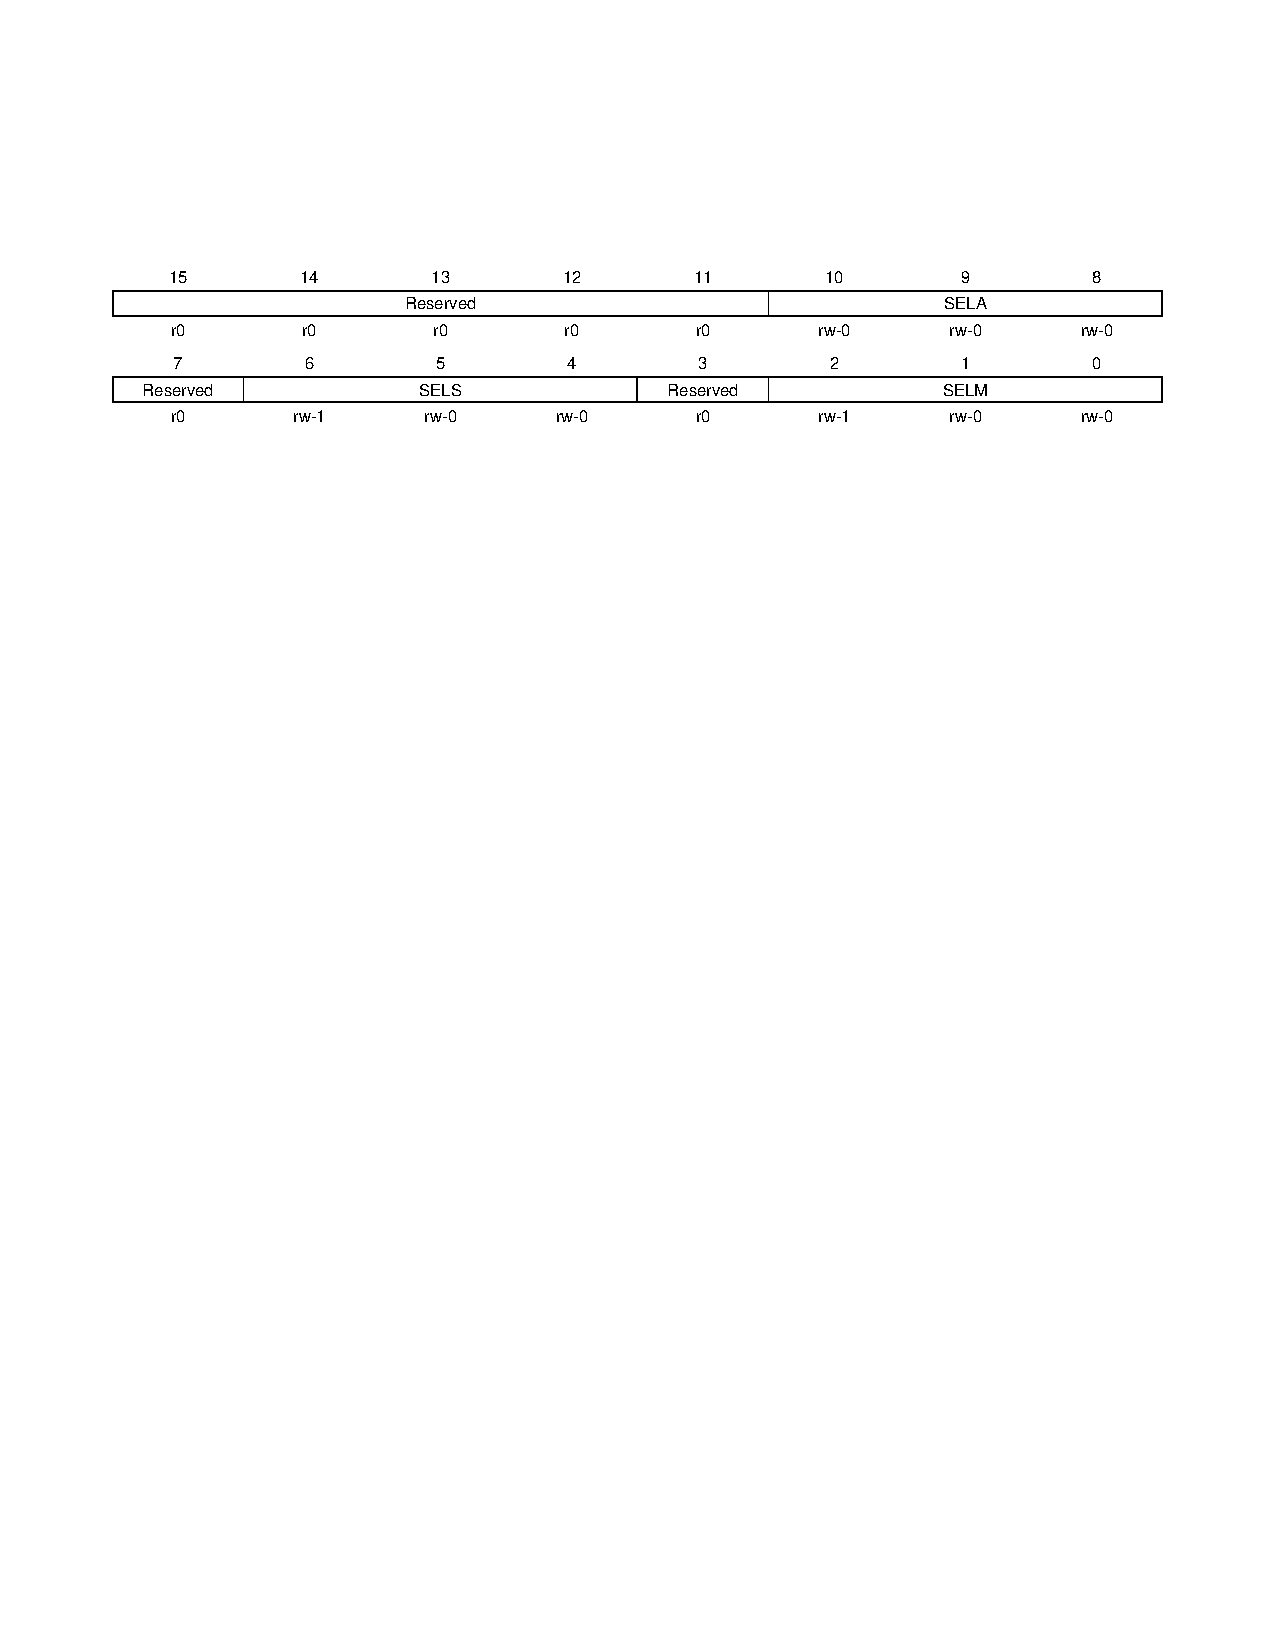
\includegraphics [angle=0, width=16cm]{./Figures/Chap6_Horloges/UCSCTL4.pdf}
  \rule{35em}{0.5pt}
  \caption{UCSCTL4}
  \label{fig:UCSCTL4}
\end{figure}

\begin{table}[H]
\centering 
\begin{tabular}{l l l l}
\hline\hline
Champ & & Valeur & Description \\ %[0.5ex]
\hline
SELA & & & Connection de ACLK  \\
& & 000 & XT1CLK \\
& & 001 & VLOCLK \\
& & 010 & REFOCLK \\
& & 011 & DCOCLK \\
& & 100 & DCOCLKDIV \\
& & 101 & XT2CLK \\
& & 110 & réservé \\
& & 111 & réservé \\
\hline
SELS & & & Connection de SMCLK  \\
& & 000 & XT1CLK \\
& & 001 & VLOCLK \\
& & 010 & REFOCLK \\
& & 011 & DCOCLK \\
& & 100 & DCOCLKDIV \\
& & 101 & XT2CLK \\
& & 110 & réservé \\
& & 111 & réservé \\
\hline
SELM & & & Connection de MCLK  \\
& & 000 & XT1CLK \\
& & 001 & VLOCLK \\
& & 010 & REFOCLK \\
& & 011 & DCOCLK \\
& & 100 & DCOCLKDIV \\
& & 101 & XT2CLK \\
& & 110 & réservé \\
& & 111 & réservé \\
\hline
\end{tabular}
\caption{UCSCTL4}
\label{table:UCSCTL4}
\end{table}

\pagebreak
\begin{figure}[H]
  \centering
  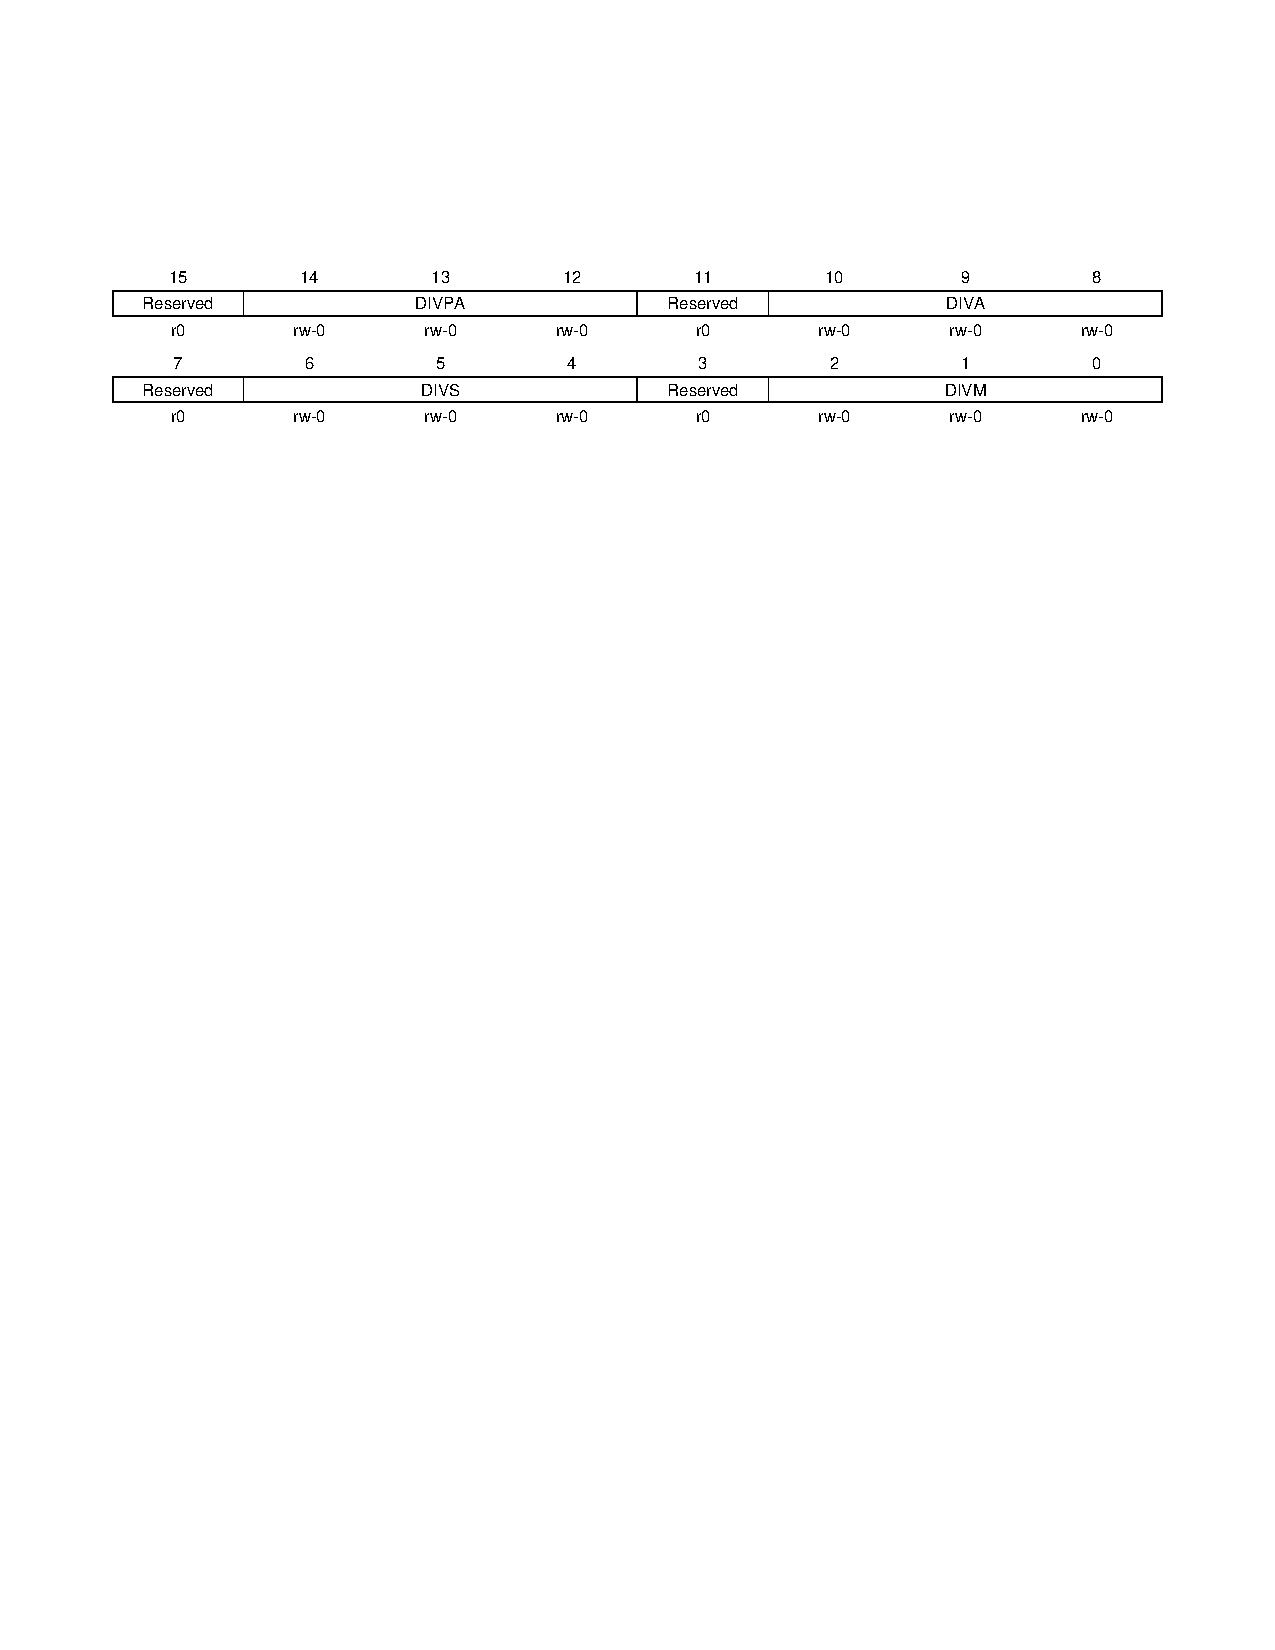
\includegraphics [angle=0, width=16cm]{./Figures/Chap6_Horloges/UCSCTL5.pdf}
  \rule{35em}{0.5pt}
  \caption{UCSCTL5}
  \label{fig:UCSCTL5}
\end{figure}

\begin{table}[H]
\centering 
\begin{tabular}{l l l l || l l l l}
\hline\hline
Champ & & Valeur & Description & Champ & & Valeur & Description \\ %[0.5ex]
\hline
DIVPA & & & génération de ACLK/n  & DIVS & & & Postdivision de SMCLK  \\
& & 000 & n = 1  & & & 000 & $f_{SMCLK}$ \\
& & 001 & n = 2  & & & 001 & $f_{SMCLK}/2$ \\
& & 010 & n = 4  & & & 010 & $f_{SMCLK}/4$ \\
& & 011 & n = 8  & & & 011 & $f_{SMCLK}/8$ \\
& & 100 & n = 16  & & & 100 & $f_{SMCLK}/16$ \\
& & 101 & n = 32  & & & 101 & $f_{SMCLK}/32$ \\
& & 110 & réservé  & & & 110 & réservé \\
& & 111 & réservé  & & & 111 & réservé \\
\hline
DIVA & & & Postdivision de ACLK  & DIVM & & & Postdivision de MCLK  \\
& & 000 & $f_{ACLK}$  & & & 000 & $f_{MCLK}$ \\
& & 001 & $f_{ACLK}/2$  & & & 001 & $f_{MCLK}/2$ \\
& & 010 & $f_{ACLK}/4$  & & & 010 & $f_{MCLK}/4$ \\
& & 011 & $f_{ACLK}/8$  & & & 011 & $f_{MCLK}/8$ \\
& & 100 & $f_{ACLK}/16$  & & & 100 & $f_{MCLK}/16$ \\
& & 101 & $f_{ACLK}/32$  & & & 101 & $f_{MCLK}/32$ \\
& & 110 & réservé  & & & 110 & réservé \\
& & 111 & réservé  & & & 111 & réservé \\
\hline
\end{tabular}
\caption{UCSCTL5}
\label{table:UCSCTL5}
\end{table}

\pagebreak
\subsection{Exemple de configuration}
Partant d'un quartz 32768 Hz connecté sur l'oscillateur XT1, le code suivant génère:
\begin{itemize}[label=\textbullet,font=\small]
\item ACLK à 327680 Hz
\item MCLK à 10,48576 MHz
\end{itemize}
Le signal ACLK est utilisé par le timer A0 pour générer des interruptions toutes les 100 ms.

\lstset{style=customc}
\begin{lstlisting}
#include <msp430.h>
int main(void) {

	// configuration du systeme d'horloge UCS
	UCSCTL1 &= ~(BIT6 | BIT5 | BIT4); // reset DCORSEL
	UCSCTL1 |= DCORSEL_5;             // range du DCO

	UCSCTL2 = 9 | FLLD__32;           // multiplication par 10 et par 32

	// XT1CLK entrée de FLL, prédivision par 1
	UCSCTL3 = SELREF__XT1CLK + FLLREFDIV__1;

	// sélection des sources pour ACLK (FXT1*10) et MCLK(FXT1*320)
	UCSCTL4 = SELA__DCOCLKDIV + SELM__DCOCLK;

	UCSCTL5 = DIVA__1;                // division de ACLK par 1

	UCSCTL6 &= ~XT1OFF;               // activation de XT1 pour ACLK

// configuration du timer A0
// génère une interruption sur CCIFG0 tous les 32768 tops
	TA0CCTL0 = CCIE;
	TA0CCR0 = 32767;
	TA0CTL = TASSEL_1 + MC_1 + TACLR;
	__enable_interrupt();
	while(1);
}

// Timer_A CCIFG0 handler
#pragma vector=TIMERA0_VECTOR
__interrupt void Timer_A (void)
{
	todo();
}
\end{lstlisting}
